\documentclass[spanish,a4paper,11pt]{book}
% \usepackage[spanish]{babel}
\usepackage[utf8]{inputenc}

\usepackage{cite} % para contraer referencias

\usepackage{listings}
\usepackage{titlesec}
\usepackage{fancyhdr}
\usepackage[spanish]{babel}
\usepackage[hidelinks]{hyperref}
\usepackage{xcolor}
\usepackage{pdfpages}
\usepackage{url}
\usepackage{booktabs}
\usepackage[export]{adjustbox}
\usepackage{fancybox}


\usepackage[backend=biber,style=ieee]{biblatex}
% \usepackage[backend=bibtex,style=verbose-trad2]{biblatex}
% \usepackage{biblatex}

\usepackage[babel]{csquotes}

\DeclareLanguageMapping{spanish-apa}

% %----------------------------------------------------------------------------------------
%	BIBLIOGRAPHY AND INDEX
%----------------------------------------------------------------------------------------
\addbibresource{bibliography/project.bib} % BibTeX bibliography file
\defbibheading{bibempty}{}


\usepackage{textcomp}

\usepackage{wrapfig}

\usepackage{blindtext}

\usepackage{float}

\usepackage{booktabs}

\usepackage{rotating}

\usepackage[hidelinks]{hyperref}

% Información reutilizable
\newcommand{\asunto}{Trabajo de Fin de Máster}
\newcommand{\titulo}{Sistema de ciberdefensa dinámica basada en algoritmos evolutivos para la prevención de ataques informáticos}
\newcommand{\tituloEng}{Evolutionary Based Moving Target Cyberdefense System}
\newcommand{\master}{Máster Profesional en Ingeniería Informática}
\newcommand{\autor}{Ernesto Serrano Collado}
\newcommand{\email}{info@ernesto.es}
\newcommand{\tutor}{Juan Julián Merelo Guervós}
\newcommand{\escuela}{Escuela Técnica Superior de Ingenierías Informática y de Telecomunicación}
\newcommand{\universidad}{Universidad de Granada}
\newcommand{\ciudad}{Granada}
\newcommand{\vers}{Versión 1.0}
\providecommand{\keywords}{seguridad informática, ciberdefensa, algoritmos genéticos, software libre}

\providecommand{\keywordsen}{computer security, cyber defense, genetic algorithms, free software}


% Información archivo
\hypersetup{
	pdfauthor = {\autor\ (\email)},
	pdftitle = {\titulo},
	pdfsubject = {\asunto},
	pdfkeywords = {\keywords},
	pdfcreator = {MacTeX con el paquete TeX Live},
	pdfproducer = {pdflatex}
}

% Estilo de cabeceras
\pagestyle{fancy}
\fancyhf{}
\fancyhead[LO]{\leftmark}
\fancyhead[RE]{\rightmark}
\fancyhead[RO,LE]{\textbf{\thepage}}
\setlength{\headheight}{1.5\headheight}

% Redefinición de comandos
\renewcommand{\lstlistingname}{Fragmento de código}
\renewcommand{\lstlistlistingname}{Índice de fragmentos de código}
\renewcommand{\chaptermark}[1]{\markboth{\textbf{#1}}{}}
\renewcommand{\sectionmark}[1]{\markright{\textbf{\thesection. #1}}}

% Definición de colores
\definecolor{gray97}{gray}{.97}
\definecolor{gray75}{gray}{.75}
\definecolor{gray45}{gray}{.45}
\definecolor{gray30}{gray}{.94}
\definecolor{lightgray}{rgb}{.9,.9,.9}
\definecolor{darkgray}{rgb}{.4,.4,.4}
\definecolor{purple}{rgb}{0.65, 0.12, 0.82}
\definecolor{background}{HTML}{EEEEEE}
\definecolor{delim}{RGB}{20,105,176}
\colorlet{punct}{red!60!black}
\colorlet{numb}{magenta!60!black}

	\definecolor{dkgreen}{rgb}{0,0.6,0}
	\definecolor{gray}{rgb}{0.5,0.5,0.5}
	\definecolor{mauve}{rgb}{0.58,0,0.82}

% Listados
\lstset{
	aboveskip=0.5cm,
	backgroundcolor=\color{gray97},
	basicstyle=\scriptsize\ttfamily,
	breaklines=true,
	%commentstyle=\color{gray45},
	frame=Ltb,
	framerule=0.5pt,
	framesep=0pt,
	framexbottommargin=3pt,
	framexleftmargin=0.1cm,
	framextopmargin=3pt,
	%keywordstyle=\bfseries,
	numberfirstline = false,
	numbers=left,
	numbersep=6pt,
	%numberstyle=\tiny,
	rulesep=.4pt,
	rulesepcolor=\color{black},
	showstringspaces = false,
	%stringstyle=\ttfamily,
	  numberstyle=\tiny\color{gray},
	  keywordstyle=\color{blue},
	  commentstyle=\color{dkgreen},
	  stringstyle=\color{mauve},
	literate={á}{{\'a}}1
	         {é}{{\'e}}1
	         {í}{{\'i}}1
	         {ó}{{\'o}}1
	         {ú}{{\'u}}1
	         {ñ}{{\~n}}1
}


% Minimizar fragmentado de listados
\lstnewenvironment{listing}[1][]
	{\lstset{#1}\pagebreak[0]}{\pagebreak[0]}

% Listado definido para JavaScript
% http://tex.stackexchange.com/questions/89574/language-option-supported-in-listings/89576#89576
\lstdefinelanguage{javascript}{
	backgroundcolor=\color{background},
	basicstyle=\footnotesize,
	breaklines=true,
	captionpos=b,
	comment=[l]{//},
	commentstyle=\color{purple}\ttfamily,
	frame=lines,
	identifierstyle=\color{black},
	keywordstyle=\color{blue}\bfseries,
	morecomment=[s]{/*}{*/},
	morestring=[b]',
	morestring=[b]",
	ndkeywordstyle=\color{darkgray}\bfseries,
	numbers=left,
	numbersep=8pt,
	numberstyle=\scriptsize,
	sensitive=false,
	showstringspaces=false,
	stepnumber=1,
	stringstyle=\color{red}\ttfamily,
	keywords={
		break,
		case,
		catch,
		catch,
		do,
		else,
		false,
		function,
		if,
		in,
		new,
		null,
		return,
		switch,
		true,
		typeof,
		var,
		while},
	ndkeywords={
		boolean,
		class,
		export,
		implements,
		import,
		this,
		throw}
}

% Listado definido para JSON
% http://tex.stackexchange.com/questions/83085/how-to-improve-listings-display-of-json-files/83100#83100
\lstdefinelanguage{json}{
	backgroundcolor=\color{background},
	basicstyle=\footnotesize,
	breaklines=true,
	captionpos=b,
	frame=lines,
	numbers=left,
	numbersep=8pt,
	numberstyle=\scriptsize,
	showstringspaces=false,
	stepnumber=1,
	literate=
		*{:}{{{\color{punct}{:}}}}{1}
		{,}{{{\color{punct}{,}}}}{1}
	    {\{}{{{\color{delim}{\{}}}}{1}
	    {\}}{{{\color{delim}{\}}}}}{1}
	    {[}{{{\color{delim}{[}}}}{1}
	    {]}{{{\color{delim}{]}}}}{1}
	    {ñ}{{\~{n}}}{1}
}

\lstdefinelanguage{yaml}{
  keywords={true,false,null,y,n},
  keywordstyle=\color{darkgray}\bfseries,
  ndkeywords={},
  ndkeywordstyle=\color{black}\bfseries,
  identifierstyle=\color{black},
  sensitive=false,
  %moredelim=[l]{}{:},
  comment=[l]{#},
  morecomment=[s]{/*}{*/},
  commentstyle=\color{purple}\ttfamily,
  stringstyle=\color{blue}\ttfamily,
  %morestring=[l]{-}{},
  morestring=[b]',
  morestring=[b]"
}

\lstdefinelanguage{docker}{
  keywords={FROM, RUN, COPY, ADD, ENTRYPOINT, CMD,  ENV, ARG, WORKDIR, EXPOSE, LABEL, USER, VOLUME, STOPSIGNAL, ONBUILD, MAINTAINER},
  keywordstyle=\color{blue}\bfseries,
  identifierstyle=\color{black},
  sensitive=false,
  comment=[l]{\#},
  commentstyle=\color{purple}\ttfamily,
  stringstyle=\color{red}\ttfamily,
  morestring=[b]',
  morestring=[b]"
}

\lstdefinelanguage{docker-compose}{
  keywords={image, environment, ports, container_name, ports, volumes, links},
  keywordstyle=\color{blue}\bfseries,
  identifierstyle=\color{black},
  sensitive=false,
  comment=[l]{\#},
  commentstyle=\color{purple}\ttfamily,
  stringstyle=\color{red}\ttfamily,
  morestring=[b]',
  morestring=[b]"
}
\lstdefinelanguage{docker-compose-2}{
  keywords={version, volumes, services},
  keywordstyle=\color{blue}\bfseries,
  keywords=[2]{image, environment, ports, container_name, ports, links, build},
  keywordstyle=[2]\color{olive}\bfseries,
  identifierstyle=\color{black},
  sensitive=false,
  comment=[l]{\#},
  commentstyle=\color{purple}\ttfamily,
  stringstyle=\color{red}\ttfamily,
  morestring=[b]',
  morestring=[b]"
}

% Para que las páginas en blanco no tengan cabecera
\makeatletter
\def\clearpage{%
  \ifvmode
    \ifnum \@dbltopnum =\m@ne
      \ifdim \pagetotal <\topskip
        \hbox{}
      \fi
    \fi
  \fi
  \newpage
  \thispagestyle{empty}
  \write\m@ne{}
  \vbox{}
  \penalty -\@Mi
}
\makeatother

\begin{document}
\begin{titlepage}

\newlength{\centeroffset}
\setlength{\centeroffset}{-0.5\oddsidemargin}
\addtolength{\centeroffset}{0.5\evensidemargin}

\noindent\hspace*{\centeroffset}\begin{minipage}{\textwidth}

\centering

\includegraphics[width=0.9\textwidth]{../images/logo_ugr.png}

\textsc{\Large\asunto\\[0.2cm]}
\textsc{\master}\\[0.5cm]

{\Huge\bfseries \titulo\\}
\noindent\rule[-1ex]{\textwidth}{3pt}\\[3.5ex]
\end{minipage}

\vspace{1cm}
\noindent\hspace*{\centeroffset}\begin{minipage}{\textwidth}
\centering

\textbf{Autor}\\ {\autor}\\[2.5ex]
\textbf{Tutor}\\ {\tutor}\\[2cm]

\includegraphics[width=0.3\textwidth]{../images/logo_etsiit.png}\\[0.1cm]
\textsc{\escuela}\\
\textsc{---}\\
\ciudad, \today\\
% 
\includegraphics[width=0.3\textwidth]{../images/CC-SA-logo.png}
\end{minipage}
\end{titlepage}
\frontmatter
\begin{center}
{\LARGE\bfseries\titulo}\\
\end{center}
\begin{center}
\autor\
\end{center}

\section*{Resumen}

\bigskip
\noindent{\textbf{Palabras clave}: \textit{\keywords}\\

Además de realizar una labor determinada de forma eficiente, los servicios informáticos deben ser capaces de evitar los ataques y de detectar los que haya. Una técnica de defensa consiste en convertirse en un objetivo móvil, que varíe el perfil de forma que los atacantes no lo reconozcan.

\bigskip
Mediante algoritmos evolutivos trataremos de configurar diferentes servicios de forma que se maximice la diversidad, a la vez que se optimice la seguridad y las prestaciones.

\newpage
\begin{center}
{\LARGE\bfseries\tituloEng}\\
\end{center}
\begin{center}
\autor\
\end{center}

\section*{Extended abstract}

\bigskip
\noindent{\textbf{Keywords}: \textit{\keywordsen}.\\

Cyber attacks are one of the biggest problems for many organizations. That organizations are investing so many resources in detecting cyber-attacks, but they still have serious difficulties to prevent them.

\bigskip
The common way to perform an attack is using a list of known vulnerabilities. Many of these vulnerabilities can be caused by a bad configuration.

\bigskip
A simple protection against computer security threats can be implemented by properly tuning existing system software without the needed of expensive security solutions.

\bigskip
This project shows a low-cost technique to prevent computer attacks. This technique consists of constantly modifying the configuration of a server.

\bigskip
Using a genetic algorithm, many different possible configurations are mutated to find an optimal solution. This optimal configuration is regularly applied, so the systems information previously collected by a potential attacker is no longer effective, achieving a simple protection layer while optimizing the service configuration.


\newpage
\thispagestyle{empty}
\
\vspace{10cm}

\noindent\rule[-1ex]{\textwidth}{2pt}\\[4.5ex]

% \section*{Declaración de Originalidad del TFM}

Yo, \textbf{\autor}, alumno de la titulación \textbf{\master} de la \textbf{\escuela\ de la \universidad}, declaro que el presente Trabajo de Fin de Máster es original, no habiéndose utilizado fuentes sin ser citadas debidamente. De no cumplir con este compromiso, soy consciente de que, de acuerdo con la Normativa de Evaluación y de Calificación de los estudiantes de la Universidad de Granada de 20 de mayo de 2013, \textit{esto conllevará automáticamente la calificación numérica de cero [...] independientemente del resto de las calificaciones que el estudiante hubiera obtenido. Esta consecuencia debe entenderse sin perjuicio de las responsabilidades disciplinarias en las que pudieran incurrir los estudiantes que plagien.}

\bigskip
Asimismo, autorizo la ubicación de la siguiente copia de mi Trabajo de Fin de Máster (\textit{\titulo}) en la biblioteca del centro para que pueda ser consultada por las personas que lo deseen.

\bigskip
Además, este mismo trabajo está publicado bajo la licencia \textbf{Creative Commons Attribution-ShareAlike 4.0} \cite{CC}, dando permiso para copiarlo y redistribuirlo en cualquier medio o formato, también de adaptarlo de la forma que se quiera, pero todo esto siempre y cuando se reconozca la autoría y se distribuya con la misma licencia que el trabajo original. Todo el código fuente así como este documento en formato {\tt LaTeX} se puede encontrar en el siguiente repositorios de {\tt GitHub}: \url{https://github.com/erseco/moving_target_defense}.

\bigskip
Y para que así conste firmo el presente documento.

\vspace{3cm}

\noindent Fdo: \autor

\vspace{3cm}

\begin{flushright}
\ciudad, a \today
\end{flushright}

\newpage
\thispagestyle{empty}
\
\vspace{3cm}

\noindent\rule[-1ex]{\textwidth}{2pt}\\[4.5ex]

D. \textbf{\tutor}, profesor del \textbf{Departamento de Arquitectura y Tecnología de los Computadores} de la \textbf{\universidad}.

\vspace{0.5cm}

\vspace{0.5cm}

\textbf{Informa:}

\vspace{0.5cm}

Que el presente trabajo, titulado \textit{\textbf{\titulo}}, ha sido realizado bajo su supervisión por \textbf{\autor}, y
autoriza la defensa de dicho trabajo ante el tribunal que corresponda.

\vspace{0.5cm}

Y para que conste, expide y firma el presente informe en \ciudad\ a \today.

\vspace{1cm}

\textbf{El tutor:}

\vspace{3cm}

%\begin{figure}[H]
%\includegraphics[width=0.3\textwidth]{../../firmaJJ}
%\end{figure}

\noindent \textbf{\tutor}

\chapter*{Agradecimientos}
\thispagestyle{empty}

\vspace{1cm}

A Georgia, que algún día será mejor ingeniera que su tío.

\bigskip
Al ZX Spectrum 128K de mis hermanos, porque sin él no habría llegado hasta aquí.


\begingroup
\let\cleardoublepage\clearpage
  \tableofcontents
%  \listoffigures
%  \listoftables
%  \lstlistoflistings
\endgroup

\newpage
\thispagestyle{empty}
\
\mainmatter
\chapter{Introducción}

\section{Motivación}

En un mundo interconectado los ciberataques son uno de los mayores problemas para muchas organizaciones. Las organizaciones cada vez invierten más recursos en la detección de ataques informáticos, pero debido al amplio espectro de los mismos todavía tenemos serias dificultades para prevenirlos.

\bigskip
Las pérdidas en la economía mundial causadas por el cibercrimen y el ciberespionaje se estiman en cientos de miles de millones de dólares\cite{herrero_cibercrimen_2015}. Según un estudio del Instituto de Investigación Interregional de Crimen y Justicia de las Naciones Unidas (UNICRI por sus siglas en inglés), el cibercrimen es una de las principales amenazas para la economía mundial pasando el coste asociado al cibercrimen de 400.000 millones de Dólares en 2014\cite{zappa_cybercrime:_2014} a alcanzar, según la Interpol, una estimacionón de 750.000 millones de Euros sólo en Europa\cite{gil_cuanto_2018}.

\bigskip
Las pérdidas estimadas causadas por actividades cibernéticas maliciosas están dentro de los siguientes criterios\cite{armin_2020_2015}:

\begin{itemize}
  \item Robo de propiedad intelectual e información comercial confidencial.
  \item Robo de información sensible, incluida la posible manipulación del mercado.
  \item Coste de oportunidad que incluye interrupciones en el servicio, y una menor confianza en las actividades en línea.
  \item Pérdida causada por daños a la reputación de los negocios pirateados.
\end{itemize}

\bigskip
La forma mas común de realizar dichos ataques es haciendo uso de vulnerabilidades conocidas. Muchas de estas vulnerabilidades pueden ser causadas por una mala configuración o por una combinación inadecuada de parámetros. Asimismo, un servicio determinado puede tener prácticamente infinitas configuraciones posibles, siendo unas menos funcionales y/o vulnerables que otras.

\bigskip
La protección contra multitud de amenazas de seguridad informática puede ser implementada mediante una correcta configuración del software existente sin necesidad de invertir en costosas soluciones de seguridad.

\bigskip
Los algoritmos genéticos, que es una heurística de búsqueda, se pueden utilizan para descubrir configuraciones de computadora nuevas, seguras y diversas mediante el modelado de una determinada configuración como si fueran cromosomas y las distintas opciones de configuración individuales como si fueran genes\cite{gensch_evolving_2016}. La idea principal de los algoritmos genéticos es que mediante mutación, cruce y selección de dichos cromosomas obtendremos mejores configuraciones. Dichas mutaciones se incorporan al azar, lo que proporciona diversidad.

\bigskip
Para mejorar el mecanismo de protección contra los ciberataques, el atacante puede ser engañado por un cambio continuo en la configuración de un determinado servicio y en el caso de que el atacante sea capaz de descubrir vulnerabilidades en un programa específico el algoritmo genético habrá cambiado la configuración antes de que el atacante pueda definir un ataque en base a las vulnerabilidades descubiertas.

\bigskip
En nuestro caso concreto, los algoritmos genéticos nos proporcionarán una mejor seguridad a través de la diversidad\cite{crouse_improving_2012}.

\bigskip
Todo el código utilizado para la realización de este proyecto así como las diferentes herramientas tienen licencias de código abierto, tanto por motivación ideológica como por seguridad, ya que diversos estudios indican que el Software Libre es mucho mas seguro que el propietario\cite{clark_is_2009}.


\section{Definición del problema}

Un atacante suele comenzar su ataque realizando un reconocimiento previo. Luego planea su ataque de acuerdo con la información que encuentra, por lo tanto, un cambio periódico en la configuración es una ingeniosa forma de hacer que su esfuerzo de reconocimiento no sea efectivo y ayudaría a prevenir un ataque a un costo relativamente bajo.

\bigskip
La técnica del ``objetivo móvil'' o ``Moving Target Defense'' es aplicable incluso a elementos hardware como se ha visto en el diseño del procesador Morpheus que es capaz de cambiar su configuración interna cada 50 milisegundos\cite{gallagher_morpheus:_2019}.

\bigskip
En nuestro caso utilizaríamos un sistema de inteligencia artificial\cite{tribak_alisis_2012} para alterar la configuración de un servidor de forma regular saboteando así los esfuerzos de recopilación de información realizados por un posible atacante.

\bigskip
Las distintas configuraciones posibles van cambiando (mutando) mediante un algoritmo genético hasta alcanzar una solución óptima. Si dichas configuraciones óptimas son aplicadas de forma regular la información recopilada previamente por un posible atacante ya no es efectiva consiguiendo una capa de protección sencilla y económica a la vez que se optimiza la configuración del servicio\cite{john_evolutionary_2014}.

\bigskip
Es importante asegurarse de que las configuraciones generadas funcionen de una manera correcta, y es importante que dicha configuración sea segura. Es difícil encontrar una configuración segura debido a la gran cantidad de configuraciones para probar, y además de eso, es difícil encontrar la combinación entre las configuraciones que hace que los componentes sean seguros. Para solucionar este problema deberemos contar con una herramienta que nos pueda indicar el nivel de seguridad de una configuración determinada.


\section{Estructura del proyecto}

\bigskip
Antes de pasar a detalles más técnicos, me gustaría detallar el contenido de este proyecto:

\begin{itemize}
  \item En el \textit{capítulo 1} (\textbf{Introducción}) se encuentra una breve introducción a nuestra idea, así como las motivaciones que nos han llevado a realizarla.
  \item El \textit{capítulo 2} (\textbf{Objetivos}) define los objetivos que se quieren alcanzar con este proyecto.
  \item En el \textit{capítulo 3} (\textbf{Antecedentes}) se analiza el estado de arte actual, así como algunas de las tecnologías y paradigmas que utilizaremos en nuestro proyecto.
  \item En el \textit{capítulo 4} (\textbf{Metodología}) está la planificación y desarrollo de cada uno de los apartados del proyecto.
  \item En el \textit{capítulo 5} (\textbf{Resultados})se detallan todos los resultados obtenidos.
  \item En el \textit{capítulo 6} (\textbf{Conclusiones}) se pueden encontrar las conclusiones finales  así como las recomendaciones para futuros trabajos.

\end{itemize}

\bigskip
Para finalizar se incluye un anexo con el código fuente desarrollado y liberado bajo la licencia libre \cite{free_software_foundation_gnu_2007}. Dicho código fuente también se puede encontrar en la url \url{https://github.com/erseco/moving_target_defense}.



% %
% % Ejemplos de codigo LaTeX para uso futuro
% %

% \begin{figure}[h!]
% \centering
% 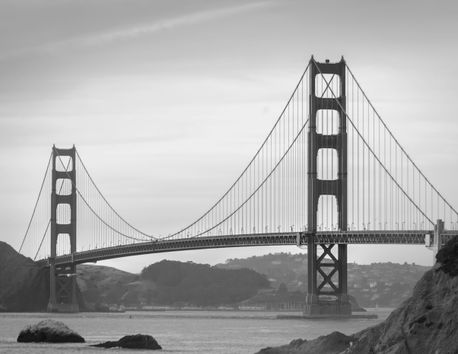
\includegraphics[width=1.0\textwidth]{../images/sample1}
% \caption{Sample Image 1}
% \label{fig:sample1}
% \end{figure}

% Esto es un texto con una nota\footnote{Ejemplo de nota al pie} al pie.

% Y esto es una ``Frase de alguien'' (\cite{john_evolutionary_2014}).

% \begin{itemize}
%   \item \textbf{1.} Texto de ejemplo
%   \item \textbf{2.} Texto de ejemplo
%   \item \textbf{3.} Texto de ejemplo
%   \item \textbf{4.} Texto de ejemplo

% \end{itemize}

% \begin{enumerate}
% 	\item Ejemplo 1.
% 	\item Ejemplo 2.
% \end{enumerate}

% \begin{lstlisting}[language=html]
% <!DOCTYPE html>
% <html lang="es-ES">
%   <head>
%     <meta charset="utf-8">
%     <title>Ejemplo de 2 párrafos</title>
%   </head>
%   <body>
%     <p>Esto es un párrafo.</p>
%     <p>Esto es otro párrafo.</p>
%   </body>
% </html>
% \end{lstlisting}

% Puedes verlo en \cite{merelo-guervos_comparison_2016}. Te recomiendo leer \cite{clark_is_2009, zhang_genetic_2009, schlenker_deceiving_2018, gensch_evolving_2016}.

\chapter{Objetivos}

Los objetivos de este proyecto son prevenir ataques informáticos utilizando la técnica del `objetivo móvil', comprobar si utilizar una heurística de búsqueda, como pueden ser los algoritmos genéticos, puede servir para generar de forma automatizada las distintas configuraciones con la suficiente diversidad atendiendo también a la seguridad del sistema a la hora de generar dichas configuraciones.

\bigskip
Para poder acometer dichos objetivos se ha optado por el desarrollo una herramienta software que mediante el uso de algoritmos genéticos sea capaz de optimizar la configuración de un determinado servicio y que, aplicando dicha configuración de forma regular, la seguridad del servicio se vea incrementada al entorpecer la recopilación de información realizada por un posible atacante \cite{john_evolutionary_2014}.

\bigskip
Para alcanzar estos objetivos realizaremos las siguientes tareas:

\begin{itemize}
  \item \textbf{TAREA-1.} Analizar distintos servicios web candidatos a ser optimizados y securizados.
  \item \textbf{TAREA-2.} Analizar las posibilidades de configuración de los servicios anteriores.
  \item \textbf{TAREA-3.} Cuantificar la seguridad de una determinada configuración.
  \item \textbf{TAREA-4.} Desarrollar una herramienta para prevenir ataques informáticos.
\end{itemize}

\section{Alcance de los objetivos}
El fin inmediato de este proyecto es conseguir prevenir ataques informáticos ayudando a los administradores de sistemas securizar servidores de una forma sencilla.

\bigskip
Además todo el código así como la documentación resultante se liberará con una licencia libre para que cualquiera pueda hacer uso de las conclusiones y los datos extraídos del análisis.

\section{Interdependencia de las tareas}

Todos las tareas son interdependientes entre sí. En aspectos más relacionados con la realización del proyecto, la tercera tarea (\textbf{TAREA-3}) la el que nos brindará el sistema sobre la que trabajar, ya que sienta la base sobre la que aplicar la cuarta tarea (\textbf{TAREA-4}). El análisis realizado en las dos primeras tareas (\textbf{TAREA-1} y \textbf{TAREA-2}) nos indicarán que servidor y herramientas podremos utilizar para realizar el resto de tareas.

\section{Conocimientos y herramientas utilizadas}

\bigskip
Destacar en los aspectos formativos previos más utilizados para el desarrollo del proyecto los conocimientos adquiridos en las asignaturas ``Cloud Computing'' para el análisis y configuración de los diferentes servicios de red así como todo lo referente a virtualización de sistemas, ``Inteligencia Computacional'' para el desarrollo del algoritmo genético y ``Planificación y Gestión de Proyectos Informáticos'' para definir los requisitos y el planteamiento inicial del proyecto, siendo todas ellas del \textbf{\master}. También destacar las asignaturas del \textbf{Grado en Ingeniería Informática} ``Seguridad en Sistemas Operativos'' para la parte de seguridad y ``Servidores Web de Altas Prestaciones'' para la realización de pruebas desde el punto de vista de disponibilidad y carga de trabajo.

\bigskip
Para la realización de cada una de las partes se han usado multitud de herramientas específicas tales como \texttt{LaTeX}, \texttt{Zotero}, \texttt{Docker} \texttt{Git} y \texttt{OWASP ZAP} entre otras.


\chapter{Antecedentes}

En este capítulo vamos analizar el estado de arte actual y las tecnologías candidatas a utilizarse en este proyecto en base a los objetivos que presentamos en el capítulo anterior.

\bigskip
Como ya vimos en la introducción, diversos estudios aseguran que es posible incrementar la seguridad de una configuración en base al uso de algoritmos genéticos, pero la mayoría son demostraciones teóricas sin ninguna implementación real cuantificable  \cite{john_evolutionary_2014} \cite{romero_sistema_2017} \cite{buji_genetic_2017}. 

\section{Herramientas existentes}
A pesar de las multiples aproximaciones teóricas \cite{schlenker_deceiving_2018} \cite{champagne_genetic_2018}, actualmente no existe ninguna herramienta, ni ningún ejemplo liberado de forma pública que permita comprobar y generar configuraciones e ir evolucionando las mismas para mejorar tanto su seguridad como su diversidad por lo que se ha optado por la realización de una herramienta capaz de realizar esto.

\bigskip
Para el análisis y cuantificación de vulnerabilidades si existe herramientas, además algunas de ellas liberadas con licencias abiertas. Hemos optado por OWASP ZAP ya que es uno de las herramientas de análisis de vulnerabilidades más utilizadas y además está liberada bajo la licencia GPLv3 \cite{free_software_foundation_gnu_2007}.

\section {Protocolos y/o servidores de red}

En esta sección analizaremos algunos de los protocolos de red más conocidos así como algunas de sus implementaciones. Ateniéndonos a la filosofía abierta de este proyecto nos limitaremos a las implementaciones libres de los mismos, además, diversas publicaciones demuestran que el software de código abierto es mas seguro que el software cerrado \cite{walia_comparative_2006} \cite{mansfield-devine_open_2008} \cite{clark_is_2009}.

\subsection {SMB - Server Message Block}

Es un protocolo de red desarrollado por IBM a principios de la década de los 90 y adoptado por Microsoft a partir de 1992. Este protocolo permite compartir archivos e impresoras en red.

\bigskip
Debido a la cantidad de sistemas compatibles es uno de los protocolos más utilizados para compartir ficheros en redes empresariales, esto hace que sea uno de los objetivos principales de muchos ciberataques.

\bigskip
Por poner un ejemplo, en mayo de 2017 hubo un ciberataque masivo causado por el ransomware WannaCry \cite{sarabia_mayor_2017}, dicho software hacía uso de un \textit{exploit} conocido como EternalBlue que conseguía penetrar en sistemas que todavía hacían uso de los protocolos SMB1 y SMB2 obligando a MicroSoft a publicar parches incluso para sistemas operativos que habían terminado su ciclo de vida (Windows XP y Windows Vista).


\subsubsection {Implementaciones libres}

\begin{table}[H]
\begin{tabular}{|l|l|}
\hline
Nombre                   & Samba                        \\ \hline
Licencia                 & GPLv3                        \\ \hline
Año de lanzamiento       & 1992                         \\ \hline
Lenguaje de programación & C++, Python y C              \\ \hline
Sitio Web                & \url{https://www.samba.org} 	\\ \hline
\end{tabular}
\caption{Ficha técnica Samba}
\end{table}

Samba es una implementación libre del protocolo usado para compartir archivos de Microsoft desarrollado originalmente para Unix por Andrew Tridgell utilizando técnicas de ingeniería inversa para averiguar el funcionamiento del protocolo. Aunque sigue siendo un protocolo propietario a partir de la versión 2.0 (2006) Microsoft comenzó a publicar las especificaciones del protocolo SMB para permitir la interoperatibilidad entre diferentes sistemas operativos.


\subsection {NTP - Network Time Protocol}

Network Time Protocol (NTP) es un protocolo utilizado para sincronizar los relojes de diversos sistemas informáticos.

\subsubsection {Implementaciones libres}

\begin{table}[H]
\begin{tabular}{|l|l|}
\hline
Nombre                   & OpenNTPD                       \\ \hline
Licencia                 & ISC                            \\ \hline
Año de lanzamiento       & 2004                           \\ \hline
Lenguaje de programación & C                              \\ \hline
Sitio Web                & \url{http://www.openntpd.org}  \\ \hline
\end{tabular}
\caption{Ficha técnica OpenNTPD}
\end{table}

OpenNTPD es una implementación del protocolo NTP para sincronizar el reloj del sistema contra servidores NTP remotos. También puede actuar como un servidor NTP para clientes compatibles con NTP. OpenNTPD está desarrollado principalmente por Henning Brauer como parte del proyecto OpenBSD.

\bigskip
La motivación para desarrollar OpenNTPD fue una combinación de problemas con las implementación NTP existentes como pueden ser una configuración difícil, código complejo y difícil de auditar así como licencias incompatibles con la licencia BSD.


\subsection {VPN - Virtual Private Network}

Una red privada virtual (VPN) es una tecnología que permite crear una red segura de acceso local (LAN) sobre una red pública como puede ser Internet.

\bigskip
El protocolo más utilizado es IPSEC, pero también existen protocolos como pueden ser PPTP y L2TP. Cada uno con sus ventajas y desventajas en cuanto a seguridad, facilidad, mantenimiento y tipos de clientes soportados.

\subsubsection {Implementaciones libres}

\begin{table}[H]
\begin{tabular}{|l|l|}
\hline
Nombre                   & strongSwan                       \\ \hline
Licencia                 & GPLv2                            \\ \hline
Año de lanzamiento       & 2005                           \\ \hline
Lenguaje de programación & C                              \\ \hline
Sitio Web                & \url{http://www.strongswan.org} \\ \hline
\end{tabular}
\caption{Ficha técnica strongSwan}
\end{table}

\begin{table}[H]
\begin{tabular}{|l|l|}
\hline
Nombre                   & Libreswan                       \\ \hline
Licencia                 & GPL                            \\ \hline
Año de lanzamiento       & 2013                           \\ \hline
Lenguaje de programación & C                              \\ \hline
Sitio Web                & \url{http://libreswan.org} \\ \hline
\end{tabular}
\caption{Ficha técnica Libreswan}
\end{table}


\subsection {SSH - Secure Shell}

El protocolo SSH (Secure SHel) sirve para abrir un intérprete de comandos en un servidor remoto.

\bigskip
Además de dicho intérprete de comandos, SSH nos permite copiar datos de forma segura (scp), gestionar claves de tipo publica/privada para no requerir el uso de contraseñas y pasar los datos de cualquier otra aplicación por un canal seguro a través de túneles.

\subsubsection {Implementaciones libres}

\begin{table}[H]
\begin{tabular}{|l|l|}
\hline
Nombre                   & Dropbear                       \\ \hline
Licencia                 & MIT                            \\ \hline
Año de lanzamiento       & 2003                           \\ \hline
Lenguaje de programación & C                              \\ \hline
Sitio Web                & \url{http://matt.ucc.asn.au/dropbear/dropbear.html} \\ \hline
\end{tabular}
\caption{Ficha técnica Dropbear}
\end{table}

Dropbear es un servidor SSH desarrollado por Matt Johnston. Está diseñado para entornos con pocos recursos como pueden ser sistemas embebidos por lo que es ampliamente utilizado en routers basados en Linux como puede ser OpenWRT.

\begin{table}[H]
\begin{tabular}{|l|l|}
\hline
Nombre                   & OpenSSH                       \\ \hline
Licencia                 & BSD                            \\ \hline
Año de lanzamiento       & 1999                           \\ \hline
Lenguaje de programación & C                              \\ \hline
Sitio Web                & \url{http://www.openssh.com} \\ \hline
\end{tabular}
\caption{Ficha técnica Libreswan}
\end{table}

OpenSSH es una implementación libre del protocolo SSH desarrollado por Theo de Raadt, fundador también del proyecto OpenBSD.

\subsection {FTP - File Transfer Protocol}

FTP (File Transfer Protocol) es uno de los primero protocolos diseñado para la transferencia de archivos entre sistemas utilizando una arquitectura cliente/servidor. A pesar de sus problemas de seguridad \cite{todd_why_2000} es uno de los protocolos más utilizados para transferir archivos. Dichos problemas se deben a que el todo el intercambio de información, desde la autenticación del usuario hasta la transferencia de, archivo, se realiza en texto plano sin ningún tipo de cifrado. Hoy en día se aconseja el uso de otros métodos mas eficaces como los programas rsync o scp basados a su vez en SSH. El propio repositorio de código de \texttt{vsftpd} fue comprometido en 2011 \cite{hkcert_security_bulletin_sa11070501_2011}.

\subsubsection {Implementaciones libres}

\begin{table}[H]
\begin{tabular}{|l|l|}
\hline
Nombre                   & vsftpd                       \\ \hline
Licencia                 & GPLv2                        \\ \hline
Año de lanzamiento       & 2001                         \\ \hline
Lenguaje de programación & C                            \\ \hline
Sitio Web                & \url{https://security.appspot.com/vsftpd.html} \\ \hline
\end{tabular}
\caption{Ficha técnica vsftp}
\end{table}

vsftpd es un servidor FTP con licencia GPL para sistemas UNIX.

\subsection {HTTP - Hypertext Transfer Protocol}

El protocolo de transferencia de hipertexto, HTTP por sus siglas en inglés, es un protocolo de red. Se utiliza para enviar y recibir páginas web en Internet. Fue desarrollado por Tim Berners-Lee y está coordinado por el \textbf{World Wide Web Consortium} (W3C).

\subsubsection {Implementaciones libres}

\begin{table}[H]
\begin{tabular}{|l|l|}
\hline
Nombre                   & Apache                       \\ \hline
Licencia                 & Apache 2.0                        \\ \hline
Año de lanzamiento       & 1995                         \\ \hline
Lenguaje de programación & C                            \\ \hline
Sitio Web                & \url{https://httpd.apache.org} \\ \hline
\end{tabular}
\caption{Ficha técnica Apache}
\end{table}

El servidor HTTP Apache es un servidor web HTTP de código abierto desarrollado y mantenido por la Fundación Apache siendo uno de los servidores HTTP más utilizados del mundo.​


\begin{table}[H]
\begin{tabular}{|l|l|}
\hline
Nombre                   & NGINX                       \\ \hline
Licencia                 & BSD                        \\ \hline
Año de lanzamiento       & 2004                        \\ \hline
Lenguaje de programación & C                            \\ \hline
Sitio Web                & \url{http://nginx.org} \\ \hline
\end{tabular}
\caption{Ficha técnica NGINX}
\end{table}

NGINX es un servidor web de alto rendimiento inicialmente desarrollado por Igor Sysoev siendo uno de los mas utilizados en la actualidad.

\section {Algoritmos genéticos}

Un algoritmo genético es un algoritmo de optimización que imita el proceso de selección natural descrito por Charles Darwin en su teoría de la evolución y nos puede ayudar a resolver problemas de optimización y búsqueda imitando procesos biológicos naturales, como pueden ser la mutación, la selección y el cruzamiento \cite{batista_algoritmos_2009}.

\bigskip
Los algoritmos genéticos son heurísticas de búsqueda que se utilizan a menudo para encontrar soluciones complejas y no obvias a la optimización algorítmica y a los problemas de búsqueda \cite{orcero_inteligencia_2002}.

\bigskip
Los algoritmos genéticos se basan en un conjunto de individuos de una población natural, codificando la información de cada solución en una cadena llamada cromosoma. Los símbolos que forman la cadena son llamados genes.

\bigskip
Los cromosomas evolucionan a través de iteraciones, llamadas generaciones. En cada generación, los cromosomas son evaluados usando alguna medida de aptitud. Las siguientes generaciones (nuevos cromosomas), son generadas aplicando los operadores genéticos de selección, mutación y cruzamiento repetidamente.



\chapter{Metodología}

En este capítulo vamos a definir y a detallar las herramientas necesarias y los procesos que vamos a seguir para solucionar el problema planteado en base a los objetivos que presentamos en el segundo capítulo y a los antecedentes vistos en el tercero.

\section{Herramientas utilizadas}

\subsection{OWASP ZAP}

Analizar la seguridad es una tarea compleja que requiere tener en cuenta multitud de factores por lo que realizar dicho análisis de forma manual resulta poco menos que imposible. Por ello vamos a utilizar \texttt{ZAP} que es un analizador de vulnerabilidades de código abierto desarrollado por la organización \texttt{OWASP}. Dicho analizador fue una de las herramientas que obtuvo el premio \textit{Bossie 2015} al mejor software de red y seguridad de código abierto \cite{staff_bossie_2015}.

\bigskip
Aunque ZAP tiene una interfaz gráfica (ver \ref{fig:owasp_zap}) para nuestro proyecto vamos a automatizar su uso mediante la API disponible en lenguaje Python.


\begin{figure}[H]
\centering
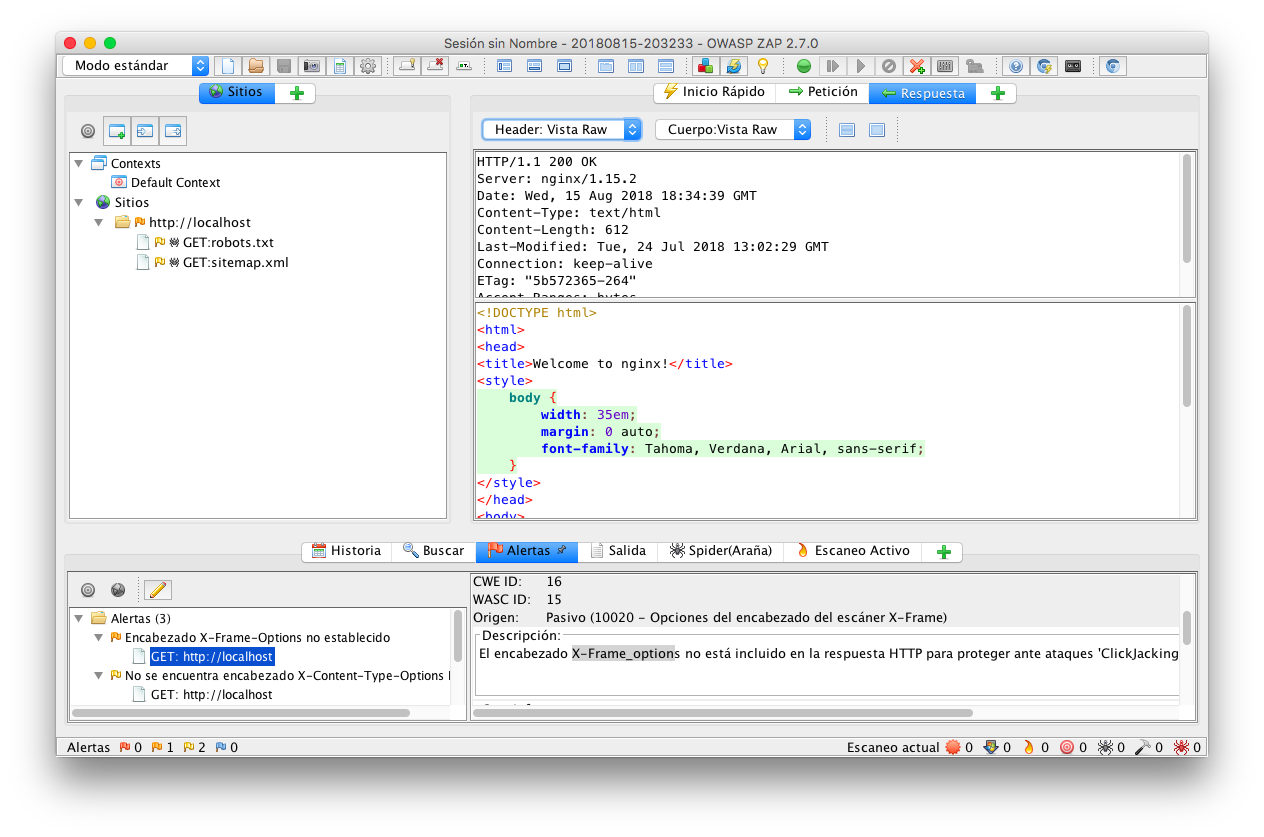
\includegraphics[width=1.0\textwidth]{../images/owasp-zap-main-window}
\caption{Ventana principal de OWASP ZAP}
\label{fig:owasp_zap}
\end{figure}


\subsection{Docker}

Para simular diferentes servidores de una forma rápida se ha optado por usar un sistema de virtualización ligera basada en contenedores. Para esto se ha usado \textfb{Docker} que es uno de los sistemas de virtualización ligera basada en contenedores más utilizada. Para la orquestación de los diferentes contenedores (Servidor y Analizador) se utilizará el estándar \textbf{docker-compose} que nos permite definir un conjunto de contenedores de una forma sencilla en un fichero de texto YML.

\bigskip
La orquestación estará compuesta de dos contenedores, uno basado en \textit{Alpine Linux} en el que instalaremos el servidor que vayamos a analizar y un segundo contenedor basado en la imagen oficial de ZAP que podemos encontrar en la URL: \url{https://hub.docker.com/r/owasp/zap2docker-bare/}.

\subsection{Python}

Se ha decidido desarrollar este proyecto en el lenguaje de programación Python debido a estar familiarizado con este lenguaje y a la disponibilidad de una API de OWASP ZAP en dicho lenguaje. Además, aunque este proyecto no requiere un elevado rendimiento, diversas publicaciones indican un muy buen desempeño del lenguaje Python a la hora de trabajar con algoritmos genéticos \cite{merelo-guervos_comparison_2016}.

\section{Análisis general del problema}

Teniendo en cuenta la ingente cantidad de servicios de red con sus múltiples opciones de configuración se ha optado por limitar este proyecto a alterar y optimizar la configuración de un servidor HTTP, concretamente NGINX ya en los últimos años ha desbancado a Apache como el servidor HTTP  más utilizado del mundo \cite{w3techs_usage_2019}.

\bigskip
La configuración de NGINX, al igual que la de muchos otros servidores, se realiza mediante ficheros de texto plano con una sintaxis específica, la misma se puede encontrar definida en la siguiente URL: \url{http://nginx.org/en/docs/beginners_guide.html#conf_structure} y consta de múltiples directivas, podemos ver un ejemplo aquí: \ref{lst:nginx_config}.

\begin{lstlisting}[label={lst:nginx_config},caption={Ejemplo de fichero de configuración de NGINX}]
user nginx;
pid /var/run/nginx.pid;
worker_processes auto;

error_log /var/log/nginx/error.log warn;
events {
    worker_connections 1024;
}
http {
    include /etc/nginx/mime.types;
    default_type application/octet-stream;
    access_log /var/log/nginx/access.log;
    sendfile on;
    keepalive_timeout 65;
    gzip on;

    server {
        listen       80;
        server_name  example.com;

        access_log  /var/log/nginx/host.access.log  main;

        location / {

            add_header X-Frame-Options "SAMEORIGIN";
            proxy_pass http://juice-shop:3000;
            root   /usr/share/nginx/html;
            index  index.html index.htm;
        }

        # redirect server error pages to the static page /50x.html
        #
        error_page   500 502 503 504  /50x.html;
        location = /50x.html {
            root   /usr/share/nginx/html;
        }

    }
}
\end{lstlisting}

Como podemos observar un fichero de configuración de NGINX tiene diferentes directivas que se pueden configurar de diferentes maneras, tanto para optimizar como para simplemente simular una configuración distinta y así hacer creer a un atacante que hemos cambiado de servidor HTTTP o incluso de servidor físico.

\section{Banco de pruebas}

Para empezar definimos un banco de pruebas para comprobar que la herramienta OWASP ZAP servía para nuestro propósito. Para ello se modificó el código de ejemplo que proporcionan para su API en Python para hacerla funcionar en un entorno de contenedores. El script (zap.py \ref{zap.py}) se conecta a una determinada URL y ejecuta una serie de comprobaciones para terminar devolviendo el número de vulnerabilidades encontradas. Dichas vulnerabilidades están basadas en la escala CVSS por lo que hay vulnerabilidades consideradas críticas y otras que son solo sugerencias.

\bigskip
A la hora de obtener una web para testear se estuvo barajando el uso de diferentes entornos web como pueden ser Galileo (Perl), WordPress (PHP), una simple web realizada en html\ref{lst:simple_html_web} e incluso una aplicación web premeditadamente vulnerable desarrollada por OWASP llamada `Juice-Shop' realizada con \textbf{Node.js} pero al final se optó por utilizar el mensaje de bienvenida de `NGINX' (ver \ref{lst:nginx_welcome_message}). La configuración estándar de NGINX con dicho mensaje nos mostraba 5 alertas \ref{lst:owas_zap_welcome_message_alerts} siendo mucho mas fácil de gestionar que las 71 que obteníamos con `Juice-Shop'.

\bigskip
Una parte muy importante para el correcto funcionamiento de OWASP ZAP fue simular un dominio, en este caso utilizamos el conocido \textfb{example.com} que es un nombre reservado por la IANA (Internet Assigned Numbers Authority) en el RFC2606 \cite{eastlake_reserved_1999}. Para hacer uso del mismo se ha optado por darle ese nombre de \textfb{host} al contenedor que levanta NGINX.


\begin{lstlisting}[language=html, label={lst:simple_html_web},caption={Web sencilla realizada en HTML puro}]
<!DOCTYPE html>
<html lang="es-ES">
  <head>
    <meta charset="utf-8">
    <title>Ejemplo de 2 párrafos</title>
  </head>
  <body>
    <p>Esto es un párrafo.</p>
    <p>Esto es otro párrafo.</p>
  </body>
</html>
\end{lstlisting}

\begin{lstlisting}[language=html, label={lst:nginx_welcome_message},caption={Mensaje de bienvenida de NGINX}]
# curl -v www.example.com
*   Trying 192.168.208.4:80...
* TCP_NODELAY set
* Connected to www.example.com (192.168.208.4) port 80 (#0)
> GET / HTTP/1.1
> Host: www.example.com
> User-Agent: curl/7.65.1
> Accept: */*
>
* Mark bundle as not supporting multiuse
< HTTP/1.1 200 OK
< Server: NGINX/1.17.2
< Date: Mon, 05 Aug 2019 13:42:32 GMT
< Content-Type: text/html
< Content-Length: 612
< Last-Modified: Tue, 23 Jul 2019 13:01:30 GMT
< Connection: keep-alive
< ETag: "5d37052a-264"
< Accept-Ranges: bytes
<
<!DOCTYPE html>
<html>
<head>
<title>Welcome to NGINX!</title>
<style>
    body {
        width: 35em;
        margin: 0 auto;
        font-family: Tahoma, Verdana, Arial, sans-serif;
    }
</style>
</head>
<body>
<h1>Welcome to NGINX!</h1>
<p>If you see this page, the NGINX web server is successfully installed and
working. Further configuration is required.</p>

<p>For online documentation and support please refer to
<a href="http://NGINX.org/">NGINX.org</a>.<br/>
Commercial support is available at
<a href="http://NGINX.com/">NGINX.com</a>.</p>

<p><em>Thank you for using NGINX.</em></p>
</body>
</html>
* Connection #0 to host www.example.com left intact
\end{lstlisting}

\begin{lstlisting}[language=json,label={lst:owas_zap_welcome_message_alerts},caption={Alerts showed with NGINX default configuration}]
[{'alert': 'Web Browser XSS Protection Not Enabled',
  'attack': '',
  'confidence': 'Medium',
  'cweid': '933',
  'description': 'Web Browser XSS Protection is not enabled, or is disabled by '
                 "the configuration of the 'X-XSS-Protection' HTTP response "
                 'header on the web server',
  'evidence': '',
  'id': '0',
  'messageId': '1',
  'method': 'GET',
  'name': 'Web Browser XSS Protection Not Enabled',
  'other': 'The X-XSS-Protection HTTP response header allows the web server to '
           "enable or disable the web browser's XSS protection mechanism. The "
           'following values would attempt to enable it: \n'
           'X-XSS-Protection: 1; mode=block\n'
           'X-XSS-Protection: 1; report=http://www.example.com/xss\n'
           'The following values would disable it:\n'
           'X-XSS-Protection: 0\n'
           'The X-XSS-Protection HTTP response header is currently supported '
           'on Internet Explorer, Chrome and Safari (WebKit).\n'
           'Note that this alert is only raised if the response body could '
           'potentially contain an XSS payload (with a text-based content '
           'type, with a non-zero length).',
  'param': 'X-XSS-Protection',
  'pluginId': '10016',
  'reference': 'https://www.owasp.org/index.php/XSS_(Cross_Site_Scripting)_Prevention_Cheat_Sheet\n'
               'https://www.veracode.com/blog/2014/03/guidelines-for-setting-security-headers/',
  'risk': 'Low',
  'solution': "Ensure that the web browser's XSS filter is enabled, by setting "
              "the X-XSS-Protection HTTP response header to '1'.",
  'sourceid': '3',
  'url': 'http://www.example.com',
  'wascid': '14'},
 {'alert': 'X-Content-Type-Options Header Missing',
  'attack': '',
  'confidence': 'Medium',
  'cweid': '16',
  'description': 'The Anti-MIME-Sniffing header X-Content-Type-Options was not '
                 "set to 'nosniff'. This allows older versions of Internet "
                 'Explorer and Chrome to perform MIME-sniffing on the response '
                 'body, potentially causing the response body to be '
                 'interpreted and displayed as a content type other than the '
                 'declared content type. Current (early 2014) and legacy '
                 'versions of Firefox will use the declared content type (if '
                 'one is set), rather than performing MIME-sniffing.',
  'evidence': '',
  'id': '1',
  'messageId': '1',
  'method': 'GET',
  'name': 'X-Content-Type-Options Header Missing',
  'other': 'This issue still applies to error type pages (401, 403, 500, etc) '
           'as those pages are often still affected by injection issues, in '
           'which case there is still concern for browsers sniffing pages away '
           'from their actual content type.\n'
           'At "High" threshold this scanner will not alert on client or '
           'server error responses.',
  'param': 'X-Content-Type-Options',
  'pluginId': '10021',
  'reference': 'http://msdn.microsoft.com/en-us/library/ie/gg622941%28v=vs.85%29.aspx\n'
               'https://www.owasp.org/index.php/List_of_useful_HTTP_headers',
  'risk': 'Low',
  'solution': 'Ensure that the application/web server sets the Content-Type '
              'header appropriately, and that it sets the '
              "X-Content-Type-Options header to 'nosniff' for all web pages.\n"
              'If possible, ensure that the end user uses a '
              'standards-compliant and modern web browser that does not '
              'perform MIME-sniffing at all, or that can be directed by the '
              'web application/web server to not perform MIME-sniffing.',
  'sourceid': '3',
  'url': 'http://www.example.com',
  'wascid': '15'},
 {'alert': 'X-Frame-Options Header Not Set',
  'attack': '',
  'confidence': 'Medium',
  'cweid': '16',
  'description': 'X-Frame-Options header is not included in the HTTP response '
                 "to protect against 'ClickJacking' attacks.",
  'evidence': '',
  'id': '2',
  'messageId': '1',
  'method': 'GET',
  'name': 'X-Frame-Options Header Not Set',
  'other': '',
  'param': 'X-Frame-Options',
  'pluginId': '10020',
  'reference': 'http://blogs.msdn.com/b/ieinternals/archive/2010/03/30/combating-clickjacking-with-x-frame-options.aspx',
  'risk': 'Medium',
  'solution': 'Most modern Web browsers support the X-Frame-Options HTTP '
              "header. Ensure it's set on all web pages returned by your site "
              '(if you expect the page to be framed only by pages on your '
              "server (e.g. it's part of a FRAMESET) then you'll want to use "
              'SAMEORIGIN, otherwise if you never expect the page to be '
              'framed, you should use DENY. ALLOW-FROM allows specific '
              'websites to frame the web page in supported web browsers).',
  'sourceid': '3',
  'url': 'http://www.example.com',
  'wascid': '15'},
 {'alert': 'Web Browser XSS Protection Not Enabled',
  'attack': '',
  'confidence': 'Medium',
  'cweid': '933',
  'description': 'Web Browser XSS Protection is not enabled, or is disabled by '
                 "the configuration of the 'X-XSS-Protection' HTTP response "
                 'header on the web server',
  'evidence': '',
  'id': '6',
  'messageId': '7',
  'method': 'GET',
  'name': 'Web Browser XSS Protection Not Enabled',
  'other': 'The X-XSS-Protection HTTP response header allows the web server to '
           "enable or disable the web browser's XSS protection mechanism. The "
           'following values would attempt to enable it: \n'
           'X-XSS-Protection: 1; mode=block\n'
           'X-XSS-Protection: 1; report=http://www.example.com/xss\n'
           'The following values would disable it:\n'
           'X-XSS-Protection: 0\n'
           'The X-XSS-Protection HTTP response header is currently supported '
           'on Internet Explorer, Chrome and Safari (WebKit).\n'
           'Note that this alert is only raised if the response body could '
           'potentially contain an XSS payload (with a text-based content '
           'type, with a non-zero length).',
  'param': 'X-XSS-Protection',
  'pluginId': '10016',
  'reference': 'https://www.owasp.org/index.php/XSS_(Cross_Site_Scripting)_Prevention_Cheat_Sheet\n'
               'https://www.veracode.com/blog/2014/03/guidelines-for-setting-security-headers/',
  'risk': 'Low',
  'solution': "Ensure that the web browser's XSS filter is enabled, by setting "
              "the X-XSS-Protection HTTP response header to '1'.",
  'sourceid': '3',
  'url': 'http://www.example.com/robots.txt',
  'wascid': '14'},
 {'alert': 'Web Browser XSS Protection Not Enabled',
  'attack': '',
  'confidence': 'Medium',
  'cweid': '933',
  'description': 'Web Browser XSS Protection is not enabled, or is disabled by '
                 "the configuration of the 'X-XSS-Protection' HTTP response "
                 'header on the web server',
  'evidence': '',
  'id': '7',
  'messageId': '8',
  'method': 'GET',
  'name': 'Web Browser XSS Protection Not Enabled',
  'other': 'The X-XSS-Protection HTTP response header allows the web server to '
           "enable or disable the web browser's XSS protection mechanism. The "
           'following values would attempt to enable it: \n'
           'X-XSS-Protection: 1; mode=block\n'
           'X-XSS-Protection: 1; report=http://www.example.com/xss\n'
           'The following values would disable it:\n'
           'X-XSS-Protection: 0\n'
           'The X-XSS-Protection HTTP response header is currently supported '
           'on Internet Explorer, Chrome and Safari (WebKit).\n'
           'Note that this alert is only raised if the response body could '
           'potentially contain an XSS payload (with a text-based content '
           'type, with a non-zero length).',
  'param': 'X-XSS-Protection',
  'pluginId': '10016',
  'reference': 'https://www.owasp.org/index.php/XSS_(Cross_Site_Scripting)_Prevention_Cheat_Sheet\n'
               'https://www.veracode.com/blog/2014/03/guidelines-for-setting-security-headers/',
  'risk': 'Low',
  'solution': "Ensure that the web browser's XSS filter is enabled, by setting "
              "the X-XSS-Protection HTTP response header to '1'.",
  'sourceid': '3',
  'url': 'http://www.example.com/sitemap.xml',
  'wascid': '14'}]
\end{lstlisting}

\bigskip
Una vez hemos generado nuestro laboratorio para pruebas y viendo que se NGINX se ejecuta correctamente pasamos a probar como va cambiando la respuestas de OWASP ZAP dependiendo de la configuración de nuestro NGINX. Para ello agregamos la cabecera \begin{verbatim}add_header X-Frame-Options "SAMEORIGIN";\end{verbatim} y ejecutamos el conjunto, dándonos 4 vulnerabilidades en lugar de las 5 anteriores. Esta prueba nos indica que efectivamente la modificación de los parámetros de NGINX puede darnos configuraciones más o menos seguras.

\section{Eligiendo los parámetros}

La última versión de NGINX (1.17.2) posee 739 directivas de configuración por lo que para simplificar nuestra tarea vamos a limitarnos a un conjunto mas pequeño de directivas (ver tabla \ref{table:apache_nginx_directives}).

\bigskip
En un primer momento pensamos en basarnos en las directivas \textfb{STIG}, pero estas directivas sólo están definidas para el servidor Apache. Por suerte al ser HTTP un estándar muchas de las directivas de Apache tienen su símil en NGINX por lo que hemos extraído un conjunto de las mas representativas y que además tuvieran su equivalente para el servidor NGINX. Las puntuaciones se basan en el sistema de puntuación CVSS de acuerdo con los resultados devueltos por ZAP con el código de prueba. También se han agregado algunas cabeceras identificativas como pueden ser la identificación del servidor (ver tabla \ref{table:ngingx_headers}) así como la directivas de compresión \texttt{gzip} para tener una mayor entropía.

\begin{table}[H]
\begin{tabular}{|l|l|l|l|}
\hline
Id & STIG ID & Configuración Apache  & Equivalente NGINX              \\ \hline
0  & V-13730 & MaxClients            & worker\_connections            \\ \hline
1  & V-13726 & KeepAliveTimeout      & keepalive\_timeout             \\ \hline
2  & V-13732 & FollowSymLinks        & disable\_symlinks              \\ \hline
3  & V-13735 & Indexes               & autoindex                      \\ \hline
4  & V-13724 & Timeout               & send\_timeout                  \\ \hline
5  & V-13738 & LimitRequestFieldsize & large\_client\_header\_buffers \\ \hline
6  & V-13736 & LimitRequestBody      & client\_max\_body\_size        \\ \hline
7  & V-6724  & ServerTokens          & server\_tokens                 \\ \hline
8  &         &                       & gzip                           \\ \hline
\end{tabular}
\label{table:apache_nginx_directives}
\caption{Lista de directivas NGINX utilizadas}
\end{table}

\begin{table}[H]
\begin{tabular}{|l|l|}
\hline
Id & Cabecera                       \\ \hline
9  & X-Frame-Options                \\ \hline
10  & X-Powered-By                   \\ \hline
11 & X-Content-Type-Options         \\ \hline
12 & Server                         \\ \hline
\end{tabular}
\label{table:ngingx_headers}
\caption{Lista de cabeceras HTTP utilizadas}
\end{table}


\bigskip
Pasamos a detallar que realiza cada directiva escogida y sus posibles valores:

\subsection{worker\_connections}

\begin{table}[H]
\begin{tabular}{|l|l|}
\hline
Sintaxis      & worker\_connections number; \\ \hline
Por defecto   & worker\_connections 512;     \\ \hline
Contexto      & events     \\ \hline
\end{tabular}
\end{table}

Establece el número máximo de conexiones simultáneas que pueden ser abiertas por un proceso de NGINX.

\bigskip
Debe tenerse en cuenta que este número incluye todas las conexiones (por ejemplo, conexiones con servidores proxy, entre otros), no sólo las conexiones con clientes. Otra consideración es que el número real de conexiones simultáneas no puede exceder el límite actual del número máximo de archivos abiertos.

\subsection{keepalive\_timeout}

\begin{table}[H]
\begin{tabular}{|l|l|}
\hline
Sintaxis      & keepalive\_timeout timeout; \\ \hline
Por defecto   & keepalive\_timeout 75s;     \\ \hline
Contexto      & http, server, location     \\ \hline
\end{tabular}
\end{table}

Establece un tiempo de espera durante el cual una conexión cliente permanecerá abierta en el lado del servidor. El valor cero deshabilita las conexiones de cliente Keep-alive. La cabecera `Keep-Alive: timeout=time' está soportada por Firefox y Chrome. Internet Explorer cierra las conexiones abiertas por sí mismo en unos 60 segundos.

\subsection{disable\_symlinks}

\begin{table}[H]
\begin{tabular}{|l|l|}
\hline
Sintaxis      & disable\_symlinks on \textbar  off; \\ \hline
Por defecto   & disable\_symlinks off;     \\ \hline
Contexto      & http, server, location     \\ \hline
\end{tabular}
\end{table}

Determina cómo se deben tratar los enlaces simbólicos al abrir archivos. Cuando está desactivado los enlaces simbólicos en la ruta de acceso están permitidos y no están marcados. Este es el comportamiento por defecto. Cuando está activado y algún componente de la ruta de acceso es un enlace simbólico, se deniega el acceso a ese archivo.

\subsection{autoindex}

\begin{table}[H]
\begin{tabular}{|l|l|}
\hline
Sintaxis      & autoindex on \textbar  off; \\ \hline
Por defecto   & autoindex off;     \\ \hline
Contexto      & http, server, location     \\ \hline
\end{tabular}
\end{table}

Cuando está activado muestra el contenido de los directorios, en caso contrario no muestra nada.

\subsection{send\_timeout}

\begin{table}[H]
\begin{tabular}{|l|l|}
\hline
Sintaxis      & send\_timeout time; \\ \hline
Por defecto   & send\_timeout 60s;     \\ \hline
Contexto      & http, server, location     \\ \hline
\end{tabular}
\end{table}

Establece el tiempo de espera para transmitir una respuesta al cliente. El tiempo de espera se establece sólo entre dos operaciones de escritura sucesivas, no para la transmisión de la respuesta completa. Si el cliente no recibe nada en este tiempo, la conexión se cierra.

\subsection{large\_client\_header\_buffers}

\begin{table}[H]
\begin{tabular}{|l|l|}
\hline
Sintaxis      & large\_client\_header\_buffers number size; \\ \hline
Por defecto   & large\_client\_header\_buffers 4 8k;     \\ \hline
Contexto      & http, server     \\ \hline
\end{tabular}
\end{table}

Establece el número máximo y el tamaño de los búferes utilizados para leer los encabezados de solicitudes de clientes grandes. Una línea de petición no puede exceder el tamaño de un búfer, o el error 414 (Request-URI Too Large) es devuelto al cliente. Un campo de encabezado de solicitud no puede exceder el tamaño de un búfer también, o el error 400 (Bad Request) es devuelto al cliente. Los búferes se asignan sólo bajo demanda. Por defecto, el tamaño del búfer es igual a 8K bytes. Si una vez finalizada la tramitación de la solicitud, la conexión pasa al estado de espera, se liberan estos búferes.

\subsection{client\_max\_body\_size}

\begin{table}[H]
\begin{tabular}{|l|l|}
\hline
Sintaxis      & client\_max\_body\_size size; \\ \hline
Por defecto   & client\_max\_body\_size 1m;     \\ \hline
Contexto      & http, server, location     \\ \hline
\end{tabular}
\end{table}

Establece el tamaño máximo permitido del cuerpo de la solicitud del cliente, especificado en el campo `Content-Length' del encabezado de la solicitud. Si el tamaño de una solicitud excede el valor configurado, el error 413 (Request Entity Too Large) se devuelve al cliente. Tenga en cuenta que los navegadores no pueden mostrar correctamente este error. Configurar el tamaño a 0 desactiva la comprobación del tamaño del cuerpo de la solicitud del cliente.

\subsection{server\_tokens}

\begin{table}[H]
\begin{tabular}{|l|l|}
\hline
Sintaxis      & server\_tokens on \textbar  off; \\ \hline
Por defecto   & server\_tokens on;     \\ \hline
Contexto      & http, server, location     \\ \hline
\end{tabular}
\end{table}

Habilita o deshabilita la emisión de la versión NGINX en las páginas de error y en el campo `Server' del encabezado de respuesta.

\subsection{gzip}

\begin{table}[H]
\begin{tabular}{|l|l|}
\hline
Sintaxis      & gzip on \textbar  off; \\ \hline
Por defecto   & gzip off;     \\ \hline
Contexto      & http, server, location     \\ \hline
\end{tabular}
\end{table}

Habilita o deshabilita la compresión de las respuestas HTTP.

\subsection{X-Frame-Options}

\begin{table}[H]
\begin{tabular}{|l|l|}
\hline
Sintaxis      & X-Frame-Options: DENY \textbar  SAMEORIGIN \textbar  ALLOW-FROM url; \\ \hline
Contexto      & server, location     \\ \hline
\end{tabular}
\end{table}

La cabecera `X-Frame-Options' puede ser usada para indicar si debería permitírsele a un navegador renderizar una página de forma embebida . Las páginas web pueden usarlo para evitar ataques de \textit{clickjacking}, asegurándose que su contenido no es embebido en otros sitios.

\subsection{X-Powered-By}

\begin{table}[H]
\begin{tabular}{|l|l|}
\hline
Sintaxis      & X-Powered-by: NGINX; \\ \hline
Contexto      & server, location     \\ \hline
\end{tabular}
\end{table}

La cabecera `X-Powered-By' se usa para especificar con que software se ha generado la respuesta por parte del servidor.

\bigskip
Se recomienda no dar información demasiado extensa en dicha cabecera ya que puede revelar detalles que pueden facilitar la tarea de encontrar y explotar fallos de seguridad.


\subsection{X-Content-Type-Options}

\begin{table}[H]
\begin{tabular}{|l|l|}
\hline
Sintaxis      & X-Content-Type-Options: nosniff; \\ \hline
Contexto      & server, location     \\ \hline
\end{tabular}
\end{table}

El encabezado HTTP de respuesta `X-Content-Type-Options' es un marcador utilizado por el servidor para indicar que los tipos \textit{MIME} anunciados en los encabezados `Content-Type' no se deben cambiar ni seguir. Esto permite desactivar el `MIME type sniffing'.

\bigskip
Introducido por Microsoft en Internet Explorer 8 e implementado paulatinamente por el resto de navegadores, ayuda a los administradores puedan bloquear el rastreo de contenido, pudiendo transformar tipos MIME no ejecutables en tipos MIME ejecutables.

\subsection{server}

\begin{table}[H]
\begin{tabular}{|l|l|}
\hline
Sintaxis      & Server: NGINX 1.12; \\ \hline
Contexto      & server, location     \\ \hline
\end{tabular}
\end{table}

La cabecera `Server' contiene la información acerca del software usado por el servidor.

\bigskip
Al igual que con la cabecera `X-Powered-By', se recomienda no dar información demasiado extensa en dicha cabecera ya que puede revelar detalles que pueden facilitar la tarea de encontrar y explotar fallos de seguridad.


\section{Generación de configuraciones}

\bigskip
Para generar las distintas configuraciones de NGINX utilizamos la librería \textfb{nginx-config-builder} desarrollada por Linkedin y licenciada bajo la BSD. Dicha librería la podemos encontrar en \url{https://github.com/linkedin/nginx-config-builder}. Haciendo uso de esta librería desarrollamos un script \ref{generate_nginx_config.py} que en base a un cromosoma generaba una configuración, sin saber todavía si dicha configuración podía funcionar o no.

\bigskip
El siguiente paso es conseguir saber primeramente si la configuración funciona y después saber si la misma configuración funcional es segura. Para lo primero el propio NGINX tiene una herramienta de comprobación de configuración, la podemos invocar con el comando \textfb{NGINX -t <archivo-configuracion.conf>}, dicha herramienta nos comprueba que la sintaxis del fichero de configuración sea correcto y NGINX pueda ejecutarse sin problemas. Para lo segundo configuraremos un servidor NGINX con dicha configuracion y haremos uso de la herramienta ZAP, para poder hacerlo de forma dinámica y sencilla utilizaremos la potencia de Docker.

\bigskip
Nuestra función de evaluación utilizará una combinación de estas dos herramientas, ya que el primero nos servirá para descartar directamente las configuraciones erróneas y la segunda nos permitirá establecer la calidad de una configuración con un valor escalar.

\section{Implementación del algoritmo genético}

La implementación del algoritmo genético utiliza una combinación de procesos de selección, cruzamiento y mutación para mejorar la solución a través de varias generaciones.
\bigskip

Aunque en un primero momento se planteó el uso de algún `framework' de algoritmos genéticos como puede ser \textfb{DEAP}, desarrollado en Python, pero se optó en su lugar por utilizar un algoritmo sencillo que cubría de sobra nuestras necesidades.

\bigskip
Para la realización del algoritmo genético hemos utilizado como base uno de los múltiples ejemplos que hay en Internet. Concretamente el del estupendo tutorial que podemos encontrar en la web \textfb{robologs.net} concretamente en esta URL: \url{https://robologs.net/2015/09/01/}.

\bigskip
El sistema está diseñado para lograr el objetivo del planteamiento del problema. En este diseño, se han desarrollado dos algoritmos y en total se han utilizado cuatro guiones en conjunto para lograr el objetivo. Para los experimentos se han utilizado una serie de herramientas. El algoritmo genético responderá a la parte principal del enunciado del problema "Cómo reforzar las vulnerabilidades de seguridad causadas por la mala configuración humana o por una cadena de configuración inadecuada". El componente y las herramientas se discuten en este capítulo. El segundo algoritmo es puntuar la idoneidad de las soluciones.

\bigskip
El algoritmo genético se encarga de llamar a los anteriores scripts para generar soluciones de seguridad. En primer lugar, inicializa las soluciones aleatorias, que luego pasan por los procesos de selección, que se describen en detalle más adelante en este capítulo. El algoritmo genético depende de la puntuación de aptitud de cada solución para ir más allá en el proceso de selección, lo que significa que es responsabilidad del algoritmo de puntuación de aptitud dar puntuaciones para las soluciones y enviarlas más allá del algoritmo genético.

\bigskip
El algoritmo de puntuación (fitness.py \ref{fitness.py}) será el responsable de proporcionar al algoritmo genético las puntuaciones de fitness de las soluciones de seguridad. El sistema de puntuación se basa en las preferencias previas de STIG, que proporciona las vulnerabilidades, que será devuelto como un valor escalar dado por ZAP.

\chapter{Resultados}

En este capítulo pasamos a detallar los resultados de todos y cada uno de los test que realizamos en base a la metodología que definimos en el capítulo anterior.

\section{Análisis inicial del sistema}

Con nuestro generador de código podemos generar configuraciones aleatorias de NGINX como la que podemos ver en el listado ver \ref{lst:nginx_config_random}. Aunque como ya hemos comentado previamente esa configuración puede ser errónea o menos segura que otra configuración también generada aleatoriamente. En este caso concreto la configuración es claramente errónea porque ha seleccionado elementos que harían que NGINX no pudiera ni siquiera inicializarse.

\bigskip
Los cromosomas representan una combinación de configuraciones que tiene un tamaño construido de acuerdo a los parámetros de las configuraciones donde un alelo o más representan un parámetro. En esta investigación, el tamaño de los cromosomas es de 13 y el total de individuos en una generación es de 20, lo que es suficiente para mantener la diversidad de los parámetros de acuerdo con el número de parámetros. El número de soluciones en una generación ha sido determinado después de muchos experimentos del algoritmo. Es posible aumentar el número de cromosomas en una generación, lo que podría aumentar la diversidad, pero eso costaría más tiempo para las pruebas.

\bigskip
Para validar que nuestros datos son correctos se han introducido algunos errores en la configuración de forma intencional. Las cabeceras `X-Frame-Options' y `X-Powered-By' contienen unos valores incorrectos al final, por lo que el gen 10 nunca podrá tener un valor de 3, asimismo el gen 11 nunca podrá tener un valor de 5. Con esto nos aseguramos que efectivamente las configuraciones incorrectas nunca serán dadas por válidas.

\bigskip
A continuación pasamos a ejecutar nuestras pruebas utilizando diferentes valores y utilizando dos funciones de cruce distintas. Una funciona de cruzamiento lo hará en un único punto aleatorio y el otro lo hará en dos.

\bigskip
Se han generado los individuos de forma aleatoria y se ha ejecutado el algoritmo genético durante las generaciones indicadas, podemos ver que hay configuraciones incorrectas (en rojo).

\bigskip
Tras cada ejecución obtenemos una configuración de NGINX que podríamos aplicar en nuestro servidor.

\bigskip
Para facilitar la interpretación de los resultados en la siguiente tabla se adjunta una tabla con la correspondencia entre el identificador y su directiva NGINX asociada.

\begin{table}[H]
\begin{tabular}{|l|l|}
\hline
\textbf{Directiva NGINX}       & \textbf{Identificador} \\ \hline
worker\_connections            & 1                      \\ \hline
keepalive\_timeout             & 2                      \\ \hline
disable\_symlinks              & 3                      \\ \hline
autoindex                      & 4                      \\ \hline
send\_timeout                  & 5                      \\ \hline
large\_client\_header\_buffers & 6                      \\ \hline
client\_max\_body\_size        & 7                      \\ \hline
server\_tokens                 & 8                      \\ \hline
gzip                           & 9                      \\ \hline
X-Frame-Options                & 10                     \\ \hline
X-Powered-By                   & 11                     \\ \hline
X-Content-Type-Options         & 12                     \\ \hline
server                         & 13                     \\ \hline
\end{tabular}
\end{table}

\section{Cruzamiento en un único punto}

\subsection{Población de 10 individuos durante 2 generaciones}
Resultados para una población de 10 individuos durante 2 generaciones:
Población inicial:
\begin{table}[H]
\begin{tabular}{|l|l|l|l|l|l|l|l|l|l|l|l|l|}
\hline
\textbf{1} & \textbf{2} & \textbf{3} & \textbf{4} & \textbf{5} & \textbf{6} & \textbf{7} & \textbf{8} & \textbf{9} & \textbf{10} & \textbf{11} & \textbf{12} & \textbf{13} \\ \hline
1884  &  75  &  1  &  1  &  0  &  805  &  1491  &  1  &  1  &  0  &  {\color[HTML]{FE0000}4}  &  1  &  1 \\ \hline
666  &  17  &  0  &  1  &  1  &  659  &  1251  &  0  &  1  &  0  &  {\color[HTML]{FE0000}5}  &  1  &  1 \\ \hline
1515  &  19  &  1  &  1  &  0  &  1104  &  1720  &  1  &  0  &  3  &  2  &  1  &  0 \\ \hline
955  &  52  &  1  &  1  &  0  &  1867  &  525  &  1  &  1  &  0  &  {\color[HTML]{FE0000}5}  &  0  &  2 \\ \hline
1916  &  110  &  1  &  0  &  1  &  846  &  619  &  0  &  1  &  2  &  2  &  0  &  0 \\ \hline
604  &  106  &  1  &  0  &  1  &  2004  &  878  &  1  &  1  &  2  &  {\color[HTML]{FE0000}4}  &  1  &  0 \\ \hline
925  &  65  &  1  &  1  &  0  &  884  &  2036  &  1  &  1  &  3  &  1  &  1  &  2 \\ \hline
889  &  13  &  1  &  1  &  1  &  1599  &  1895  &  0  &  1  &  1  &  2  &  0  &  2 \\ \hline
1324  &  92  &  1  &  1  &  1  &  2009  &  692  &  0  &  1  &  2  &  1  &  0  &  1 \\ \hline
764  &  14  &  1  &  1  &  1  &  1076  &  1936  &  0  &  0  &  1  &  {\color[HTML]{FE0000}4}  &  1  &  2 \\ \hline
\end{tabular}
\end{table}
Población final:
\begin{table}[H]
\begin{tabular}{|l|l|l|l|l|l|l|l|l|l|l|l|l|}
\hline
\textbf{1} & \textbf{2} & \textbf{3} & \textbf{4} & \textbf{5} & \textbf{6} & \textbf{7} & \textbf{8} & \textbf{9} & \textbf{10} & \textbf{11} & \textbf{12} & \textbf{13} \\ \hline
1324  &  92  &  0  &  1  &  1  &  659  &  1251  &  0  &  1  &  0  &  {\color[HTML]{FE0000}5}  &  1  &  1 \\ \hline
604  &  106  &  1  &  0  &  1  &  2004  &  878  &  1  &  1  &  0  &  1  &  0  &  1 \\ \hline
666  &  17  &  0  &  0  &  1  &  846  &  619  &  0  &  1  &  2  &  2  &  0  &  0 \\ \hline
666  &  17  &  0  &  0  &  1  &  2009  &  692  &  0  &  1  &  0  &  2  &  0  &  0 \\ \hline
666  &  17  &  0  &  0  &  1  &  846  &  619  &  0  &  1  &  2  &  1  &  0  &  1 \\ \hline
666  &  17  &  0  &  1  &  1  &  2009  &  692  &  0  &  1  &  0  &  1  &  0  &  1 \\ \hline
666  &  17  &  0  &  1  &  1  &  659  &  1251  &  0  &  1  &  0  &  {\color[HTML]{FE0000}5}  &  1  &  1 \\ \hline
666  &  17  &  0  &  0  &  1  &  846  &  619  &  0  &  1  &  2  &  2  &  0  &  0 \\ \hline
604  &  106  &  1  &  0  &  1  &  2004  &  878  &  1  &  1  &  2  &  {\color[HTML]{FE0000}4}  &  1  &  0 \\ \hline
1324  &  92  &  1  &  1  &  1  &  2009  &  692  &  0  &  1  &  2  &  1  &  0  &  1 \\ \hline
\end{tabular}
\end{table}

\subsection{Población de 10 individuos durante 5 generaciones}
Resultados para una población de 10 individuos durante 5 generaciones:
Población inicial:
\begin{table}[H]
\begin{tabular}{|l|l|l|l|l|l|l|l|l|l|l|l|l|}
\hline
\textbf{1} & \textbf{2} & \textbf{3} & \textbf{4} & \textbf{5} & \textbf{6} & \textbf{7} & \textbf{8} & \textbf{9} & \textbf{10} & \textbf{11} & \textbf{12} & \textbf{13} \\ \hline
808  &  90  &  1  &  0  &  1  &  1675  &  1228  &  0  &  0  &  0  &  3  &  1  &  0 \\ \hline
1130  &  102  &  0  &  1  &  1  &  1347  &  1232  &  1  &  0  &  3  &  2  &  1  &  1 \\ \hline
886  &  81  &  0  &  0  &  1  &  1860  &  1851  &  0  &  1  &  3  &  {\color[HTML]{FE0000}5}  &  1  &  1 \\ \hline
1845  &  92  &  1  &  1  &  1  &  1978  &  1661  &  1  &  0  &  3  &  0  &  0  &  1 \\ \hline
1394  &  44  &  1  &  1  &  1  &  1986  &  975  &  0  &  1  &  0  &  3  &  0  &  1 \\ \hline
1444  &  73  &  1  &  1  &  1  &  1364  &  1532  &  0  &  1  &  0  &  {\color[HTML]{FE0000}5}  &  1  &  1 \\ \hline
960  &  22  &  1  &  0  &  0  &  780  &  1749  &  1  &  0  &  3  &  3  &  0  &  0 \\ \hline
1663  &  12  &  1  &  1  &  0  &  538  &  1004  &  0  &  1  &  3  &  2  &  0  &  0 \\ \hline
877  &  18  &  1  &  0  &  1  &  972  &  1588  &  1  &  0  &  1  &  1  &  0  &  2 \\ \hline
852  &  23  &  1  &  1  &  0  &  1881  &  1253  &  1  &  0  &  0  &  2  &  1  &  1 \\ \hline
\end{tabular}
\end{table}
Población final:
\begin{table}[H]
\begin{tabular}{|l|l|l|l|l|l|l|l|l|l|l|l|l|}
\hline
\textbf{1} & \textbf{2} & \textbf{3} & \textbf{4} & \textbf{5} & \textbf{6} & \textbf{7} & \textbf{8} & \textbf{9} & \textbf{10} & \textbf{11} & \textbf{12} & \textbf{13} \\ \hline
808  &  90  &  1  &  1  &  0  &  1675  &  1228  &  0  &  0  &  0  &  3  &  1  &  1 \\ \hline
808  &  90  &  1  &  1  &  0  &  1675  &  1228  &  0  &  0  &  0  &  3  &  1  &  0 \\ \hline
808  &  23  &  1  &  0  &  1  &  1675  &  1228  &  0  &  0  &  0  &  3  &  0  &  1 \\ \hline
808  &  23  &  1  &  0  &  0  &  1675  &  1228  &  0  &  0  &  0  &  3  &  0  &  1 \\ \hline
808  &  90  &  1  &  0  &  0  &  1675  &  1228  &  0  &  0  &  0  &  3  &  1  &  0 \\ \hline
808  &  23  &  1  &  0  &  0  &  1675  &  1228  &  0  &  0  &  0  &  3  &  1  &  0 \\ \hline
852  &  23  &  1  &  0  &  1  &  1675  &  1228  &  0  &  0  &  0  &  3  &  1  &  0 \\ \hline
852  &  23  &  1  &  0  &  1  &  1675  &  1228  &  0  &  0  &  0  &  3  &  0  &  1 \\ \hline
808  &  90  &  1  &  1  &  0  &  1675  &  1228  &  0  &  0  &  0  &  3  &  1  &  1 \\ \hline
808  &  90  &  1  &  1  &  0  &  1675  &  1228  &  0  &  0  &  0  &  3  &  1  &  1 \\ \hline
\end{tabular}
\end{table}

\subsection{Población de 20 individuos durante 20 generaciones}
Resultados para una población de 20 individuos durante 20 generaciones:
Población inicial:
\begin{table}[H]
\begin{tabular}{|l|l|l|l|l|l|l|l|l|l|l|l|l|}
\hline
\textbf{1} & \textbf{2} & \textbf{3} & \textbf{4} & \textbf{5} & \textbf{6} & \textbf{7} & \textbf{8} & \textbf{9} & \textbf{10} & \textbf{11} & \textbf{12} & \textbf{13} \\ \hline
1243  &  104  &  0  &  0  &  1  &  1308  &  1083  &  1  &  1  &  0  &  1  &  0  &  1 \\ \hline
821  &  90  &  0  &  1  &  0  &  1669  &  1685  &  1  &  0  &  3  &  {\color[HTML]{FE0000}4}  &  0  &  1 \\ \hline
729  &  31  &  0  &  1  &  1  &  1548  &  1278  &  1  &  0  &  1  &  1  &  0  &  2 \\ \hline
1265  &  11  &  1  &  1  &  0  &  1906  &  1049  &  1  &  1  &  2  &  {\color[HTML]{FE0000}4}  &  0  &  2 \\ \hline
831  &  10  &  1  &  1  &  0  &  1095  &  917  &  0  &  1  &  0  &  2  &  1  &  0 \\ \hline
1174  &  11  &  1  &  1  &  1  &  1049  &  1728  &  0  &  0  &  1  &  1  &  1  &  0 \\ \hline
832  &  56  &  0  &  0  &  0  &  1942  &  1548  &  1  &  0  &  3  &  2  &  1  &  1 \\ \hline
935  &  100  &  0  &  0  &  0  &  1562  &  1395  &  0  &  0  &  1  &  0  &  1  &  1 \\ \hline
1886  &  64  &  1  &  1  &  1  &  1533  &  1351  &  0  &  0  &  0  &  0  &  0  &  2 \\ \hline
724  &  70  &  0  &  0  &  1  &  831  &  1710  &  0  &  1  &  2  &  3  &  1  &  1 \\ \hline
519  &  44  &  1  &  0  &  1  &  1340  &  1555  &  1  &  0  &  2  &  0  &  1  &  1 \\ \hline
923  &  85  &  0  &  1  &  0  &  1910  &  1432  &  0  &  0  &  1  &  2  &  0  &  0 \\ \hline
667  &  60  &  1  &  0  &  1  &  1692  &  1686  &  1  &  1  &  0  &  0  &  1  &  0 \\ \hline
1959  &  15  &  0  &  1  &  1  &  1733  &  1242  &  1  &  1  &  3  &  0  &  0  &  2 \\ \hline
765  &  32  &  0  &  0  &  0  &  1442  &  1625  &  1  &  1  &  1  &  1  &  0  &  2 \\ \hline
1482  &  117  &  1  &  0  &  1  &  595  &  1477  &  1  &  0  &  0  &  {\color[HTML]{FE0000}5}  &  1  &  1 \\ \hline
1091  &  35  &  0  &  1  &  0  &  1389  &  2043  &  1  &  0  &  2  &  3  &  1  &  2 \\ \hline
524  &  79  &  0  &  1  &  0  &  1019  &  1730  &  0  &  0  &  3  &  {\color[HTML]{FE0000}5}  &  0  &  1 \\ \hline
1499  &  10  &  0  &  0  &  1  &  1042  &  1140  &  1  &  1  &  3  &  1  &  1  &  2 \\ \hline
966  &  12  &  1  &  0  &  0  &  1651  &  632  &  0  &  1  &  2  &  {\color[HTML]{FE0000}4}  &  0  &  0 \\ \hline
\end{tabular}
\end{table}
Población final:
\begin{table}[H]
\begin{tabular}{|l|l|l|l|l|l|l|l|l|l|l|l|l|}
\hline
\textbf{1} & \textbf{2} & \textbf{3} & \textbf{4} & \textbf{5} & \textbf{6} & \textbf{7} & \textbf{8} & \textbf{9} & \textbf{10} & \textbf{11} & \textbf{12} & \textbf{13} \\ \hline
524  &  18  &  0  &  0  &  0  &  1340  &  1686  &  0  &  1  &  0  &  0  &  1  &  0 \\ \hline
865  &  18  &  0  &  0  &  0  &  1340  &  1686  &  1  &  1  &  0  &  0  &  1  &  0 \\ \hline
524  &  39  &  0  &  0  &  0  &  1340  &  552  &  1  &  1  &  0  &  0  &  1  &  0 \\ \hline
524  &  39  &  0  &  0  &  0  &  1340  &  1686  &  0  &  1  &  0  &  2  &  1  &  0 \\ \hline
524  &  39  &  0  &  0  &  0  &  1340  &  1686  &  0  &  1  &  0  &  0  &  0  &  0 \\ \hline
524  &  40  &  0  &  0  &  0  &  1340  &  1686  &  1  &  1  &  0  &  0  &  1  &  0 \\ \hline
524  &  39  &  0  &  0  &  0  &  1340  &  1686  &  0  &  1  &  3  &  0  &  1  &  0 \\ \hline
524  &  34  &  0  &  0  &  0  &  1340  &  1686  &  0  &  1  &  0  &  0  &  1  &  0 \\ \hline
524  &  18  &  0  &  0  &  0  &  1340  &  1686  &  0  &  1  &  0  &  0  &  1  &  0 \\ \hline
806  &  34  &  0  &  0  &  0  &  1340  &  1686  &  0  &  1  &  0  &  0  &  1  &  0 \\ \hline
524  &  39  &  0  &  0  &  0  &  1340  &  1686  &  1  &  1  &  0  &  0  &  1  &  0 \\ \hline
524  &  18  &  0  &  0  &  0  &  1340  &  1952  &  0  &  1  &  0  &  0  &  1  &  0 \\ \hline
524  &  34  &  0  &  0  &  0  &  1340  &  1686  &  1  &  1  &  0  &  0  &  1  &  0 \\ \hline
767  &  39  &  0  &  0  &  0  &  1340  &  1686  &  1  &  1  &  0  &  0  &  1  &  0 \\ \hline
524  &  18  &  0  &  0  &  0  &  1340  &  1686  &  1  &  1  &  0  &  0  &  1  &  0 \\ \hline
524  &  39  &  0  &  0  &  0  &  1340  &  1686  &  1  &  1  &  0  &  0  &  1  &  0 \\ \hline
524  &  39  &  0  &  0  &  0  &  1340  &  1686  &  0  &  1  &  0  &  0  &  1  &  0 \\ \hline
524  &  39  &  0  &  0  &  0  &  1340  &  552  &  1  &  1  &  0  &  0  &  1  &  0 \\ \hline
524  &  34  &  0  &  0  &  0  &  1340  &  1686  &  1  &  1  &  0  &  0  &  1  &  0 \\ \hline
524  &  18  &  0  &  0  &  0  &  1340  &  1686  &  0  &  1  &  0  &  0  &  1  &  0 \\ \hline
\end{tabular}
\end{table}

\section{Cruzamiento en dos puntos}

\subsection{Población de 10 individuos durante 2 generaciones}
Resultados para una población de 10 individuos durante 2 generaciones:
Población inicial:
\begin{table}[H]
\begin{tabular}{|l|l|l|l|l|l|l|l|l|l|l|l|l|}
\hline
\textbf{1} & \textbf{2} & \textbf{3} & \textbf{4} & \textbf{5} & \textbf{6} & \textbf{7} & \textbf{8} & \textbf{9} & \textbf{10} & \textbf{11} & \textbf{12} & \textbf{13} \\ \hline
1997  &  107  &  0  &  1  &  0  &  1571  &  608  &  1  &  1  &  0  &  1  &  0  &  0 \\ \hline
1879  &  23  &  1  &  1  &  0  &  1378  &  1842  &  0  &  1  &  0  &  2  &  0  &  0 \\ \hline
1036  &  79  &  1  &  1  &  1  &  1687  &  763  &  1  &  0  &  3  &  {\color[HTML]{FE0000}4}  &  1  &  2 \\ \hline
1991  &  20  &  1  &  0  &  0  &  747  &  1662  &  1  &  1  &  1  &  0  &  0  &  2 \\ \hline
1793  &  43  &  0  &  0  &  0  &  1080  &  1822  &  1  &  0  &  0  &  0  &  0  &  0 \\ \hline
1471  &  81  &  0  &  1  &  0  &  1547  &  1390  &  1  &  0  &  2  &  {\color[HTML]{FE0000}5}  &  0  &  2 \\ \hline
1923  &  36  &  1  &  0  &  1  &  1269  &  717  &  0  &  0  &  1  &  {\color[HTML]{FE0000}4}  &  0  &  1 \\ \hline
961  &  47  &  1  &  0  &  1  &  634  &  1765  &  0  &  0  &  3  &  {\color[HTML]{FE0000}4}  &  0  &  0 \\ \hline
899  &  30  &  0  &  0  &  1  &  992  &  1202  &  0  &  1  &  1  &  2  &  0  &  2 \\ \hline
1423  &  78  &  0  &  1  &  0  &  1615  &  2027  &  0  &  0  &  0  &  {\color[HTML]{FE0000}5}  &  1  &  0 \\ \hline
\end{tabular}
\end{table}
Población final:
\begin{table}[H]
\begin{tabular}{|l|l|l|l|l|l|l|l|l|l|l|l|l|}
\hline
\textbf{1} & \textbf{2} & \textbf{3} & \textbf{4} & \textbf{5} & \textbf{6} & \textbf{7} & \textbf{8} & \textbf{9} & \textbf{10} & \textbf{11} & \textbf{12} & \textbf{13} \\ \hline
899  &  34  &  0  &  0  &  1  &  634  &  1765  &  0  &  0  &  0  &  1  &  0  &  1 \\ \hline
961  &  47  &  1  &  0  &  1  &  634  &  1765  &  0  &  0  &  3  &  {\color[HTML]{FE0000}4}  &  0  &  0 \\ \hline
961  &  47  &  1  &  0  &  1  &  634  &  1765  &  0  &  0  &  1  &  2  &  0  &  0 \\ \hline
899  &  47  &  1  &  0  &  1  &  634  &  1765  &  0  &  1  &  0  &  1  &  0  &  1 \\ \hline
961  &  47  &  1  &  0  &  1  &  634  &  1765  &  0  &  0  &  2  &  {\color[HTML]{FE0000}4}  &  0  &  0 \\ \hline
961  &  47  &  1  &  0  &  1  &  634  &  1765  &  0  &  0  &  3  &  {\color[HTML]{FE0000}4}  &  0  &  0 \\ \hline
961  &  47  &  1  &  0  &  1  &  634  &  1765  &  0  &  0  &  3  &  {\color[HTML]{FE0000}4}  &  0  &  0 \\ \hline
961  &  47  &  1  &  0  &  1  &  634  &  1765  &  0  &  0  &  3  &  {\color[HTML]{FE0000}4}  &  0  &  0 \\ \hline
899  &  30  &  0  &  0  &  1  &  992  &  1202  &  0  &  1  &  1  &  2  &  0  &  2 \\ \hline
899  &  30  &  0  &  0  &  1  &  992  &  1202  &  0  &  1  &  0  &  1  &  0  &  1 \\ \hline
\end{tabular}
\end{table}

\subsection{Población de 10 individuos durante 5 generaciones}
Resultados para una población de 10 individuos durante 5 generaciones:
Población inicial:
\begin{table}[H]
\begin{tabular}{|l|l|l|l|l|l|l|l|l|l|l|l|l|}
\hline
\textbf{1} & \textbf{2} & \textbf{3} & \textbf{4} & \textbf{5} & \textbf{6} & \textbf{7} & \textbf{8} & \textbf{9} & \textbf{10} & \textbf{11} & \textbf{12} & \textbf{13} \\ \hline
2008  &  57  &  1  &  1  &  0  &  1008  &  1736  &  1  &  0  &  2  &  3  &  0  &  0 \\ \hline
2036  &  115  &  1  &  1  &  0  &  715  &  1646  &  0  &  0  &  0  &  3  &  0  &  2 \\ \hline
806  &  10  &  0  &  0  &  1  &  763  &  1061  &  0  &  1  &  0  &  0  &  1  &  2 \\ \hline
1184  &  19  &  0  &  0  &  0  &  687  &  1944  &  0  &  0  &  0  &  3  &  1  &  2 \\ \hline
1244  &  100  &  0  &  0  &  1  &  1930  &  1088  &  0  &  0  &  0  &  1  &  0  &  2 \\ \hline
1498  &  46  &  0  &  1  &  0  &  819  &  1391  &  0  &  0  &  1  &  1  &  0  &  2 \\ \hline
2037  &  120  &  1  &  1  &  1  &  1137  &  1059  &  1  &  0  &  2  &  2  &  0  &  1 \\ \hline
1171  &  118  &  0  &  0  &  1  &  1564  &  569  &  0  &  1  &  1  &  {\color[HTML]{FE0000}4}  &  1  &  2 \\ \hline
714  &  120  &  1  &  0  &  0  &  1282  &  1579  &  0  &  1  &  2  &  1  &  1  &  2 \\ \hline
1710  &  87  &  0  &  0  &  0  &  654  &  529  &  0  &  0  &  2  &  1  &  1  &  2 \\ \hline
\end{tabular}
\end{table}
Población final:
\begin{table}[H]
\begin{tabular}{|l|l|l|l|l|l|l|l|l|l|l|l|l|}
\hline
\textbf{1} & \textbf{2} & \textbf{3} & \textbf{4} & \textbf{5} & \textbf{6} & \textbf{7} & \textbf{8} & \textbf{9} & \textbf{10} & \textbf{11} & \textbf{12} & \textbf{13} \\ \hline
714  &  120  &  0  &  0  &  0  &  687  &  1944  &  1  &  1  &  2  &  1  &  1  &  2 \\ \hline
714  &  43  &  0  &  0  &  0  &  1282  &  1944  &  0  &  0  &  2  &  1  &  1  &  0 \\ \hline
714  &  43  &  0  &  0  &  0  &  1282  &  1944  &  1  &  0  &  2  &  1  &  1  &  2 \\ \hline
714  &  120  &  0  &  0  &  0  &  1282  &  1579  &  0  &  1  &  1  &  1  &  1  &  0 \\ \hline
714  &  120  &  0  &  0  &  0  &  687  &  1579  &  1  &  1  &  2  &  1  &  1  &  2 \\ \hline
714  &  120  &  0  &  0  &  0  &  1282  &  1579  &  0  &  1  &  2  &  1  &  1  &  0 \\ \hline
714  &  120  &  0  &  0  &  0  &  687  &  1944  &  1  &  1  &  2  &  1  &  1  &  2 \\ \hline
714  &  43  &  0  &  0  &  0  &  1282  &  1579  &  0  &  0  &  2  &  1  &  1  &  2 \\ \hline
714  &  120  &  1  &  0  &  1  &  687  &  1944  &  1  &  0  &  2  &  1  &  1  &  2 \\ \hline
714  &  120  &  0  &  0  &  0  &  1282  &  1579  &  0  &  1  &  2  &  1  &  1  &  2 \\ \hline
\end{tabular}
\end{table}

\subsection{Población de 20 individuos durante 20 generaciones}
Resultados para una población de 20 individuos durante 20 generaciones:
Población inicial:
\begin{table}[H]
\begin{tabular}{|l|l|l|l|l|l|l|l|l|l|l|l|l|}
\hline
\textbf{1} & \textbf{2} & \textbf{3} & \textbf{4} & \textbf{5} & \textbf{6} & \textbf{7} & \textbf{8} & \textbf{9} & \textbf{10} & \textbf{11} & \textbf{12} & \textbf{13} \\ \hline
1677  &  14  &  0  &  1  &  0  &  804  &  1001  &  1  &  0  &  0  &  0  &  0  &  0 \\ \hline
1591  &  95  &  1  &  1  &  0  &  550  &  1731  &  0  &  0  &  1  &  0  &  0  &  2 \\ \hline
776  &  110  &  1  &  0  &  1  &  1205  &  1182  &  1  &  0  &  3  &  3  &  1  &  0 \\ \hline
1200  &  71  &  1  &  1  &  1  &  1903  &  1979  &  1  &  1  &  1  &  2  &  0  &  1 \\ \hline
1961  &  28  &  0  &  0  &  1  &  1211  &  1485  &  1  &  1  &  0  &  {\color[HTML]{FE0000}4}  &  0  &  2 \\ \hline
942  &  10  &  0  &  1  &  1  &  1446  &  1525  &  1  &  0  &  0  &  1  &  0  &  1 \\ \hline
537  &  48  &  1  &  0  &  1  &  1358  &  1930  &  1  &  0  &  3  &  1  &  1  &  1 \\ \hline
1105  &  10  &  1  &  0  &  0  &  571  &  1297  &  0  &  1  &  0  &  3  &  1  &  2 \\ \hline
1331  &  84  &  1  &  0  &  0  &  748  &  1126  &  0  &  0  &  2  &  {\color[HTML]{FE0000}5}  &  1  &  2 \\ \hline
2017  &  112  &  1  &  1  &  0  &  910  &  737  &  1  &  1  &  3  &  2  &  1  &  1 \\ \hline
770  &  96  &  0  &  0  &  1  &  1257  &  1804  &  1  &  1  &  1  &  3  &  0  &  1 \\ \hline
1569  &  104  &  1  &  1  &  1  &  713  &  671  &  0  &  0  &  0  &  3  &  0  &  1 \\ \hline
1280  &  120  &  1  &  1  &  1  &  1461  &  1404  &  1  &  1  &  0  &  1  &  0  &  1 \\ \hline
898  &  92  &  1  &  0  &  0  &  1943  &  1409  &  1  &  1  &  0  &  1  &  1  &  1 \\ \hline
1632  &  70  &  1  &  0  &  0  &  1821  &  1836  &  1  &  0  &  1  &  {\color[HTML]{FE0000}5}  &  0  &  1 \\ \hline
982  &  36  &  0  &  1  &  1  &  1462  &  1446  &  1  &  0  &  1  &  1  &  1  &  2 \\ \hline
1843  &  118  &  0  &  0  &  1  &  697  &  828  &  1  &  0  &  1  &  {\color[HTML]{FE0000}4}  &  0  &  0 \\ \hline
782  &  109  &  1  &  0  &  1  &  524  &  1928  &  1  &  1  &  1  &  {\color[HTML]{FE0000}4}  &  1  &  2 \\ \hline
1779  &  10  &  1  &  0  &  0  &  1627  &  1315  &  1  &  1  &  1  &  1  &  0  &  2 \\ \hline
1927  &  21  &  1  &  0  &  0  &  771  &  576  &  1  &  1  &  2  &  2  &  1  &  0 \\ \hline
\end{tabular}
\end{table}
Población final:
\begin{table}[H]
\begin{tabular}{|l|l|l|l|l|l|l|l|l|l|l|l|l|}
\hline
\textbf{1} & \textbf{2} & \textbf{3} & \textbf{4} & \textbf{5} & \textbf{6} & \textbf{7} & \textbf{8} & \textbf{9} & \textbf{10} & \textbf{11} & \textbf{12} & \textbf{13} \\ \hline
537  &  10  &  0  &  0  &  0  &  571  &  994  &  1  &  0  &  0  &  3  &  0  &  0 \\ \hline
537  &  10  &  0  &  0  &  0  &  571  &  994  &  0  &  0  &  0  &  3  &  0  &  0 \\ \hline
537  &  10  &  0  &  0  &  0  &  571  &  849  &  0  &  0  &  0  &  3  &  0  &  0 \\ \hline
537  &  10  &  0  &  0  &  0  &  571  &  994  &  0  &  0  &  0  &  3  &  0  &  0 \\ \hline
537  &  10  &  0  &  0  &  0  &  571  &  994  &  0  &  0  &  0  &  3  &  0  &  0 \\ \hline
537  &  10  &  0  &  0  &  0  &  571  &  994  &  0  &  0  &  1  &  3  &  0  &  0 \\ \hline
537  &  10  &  0  &  0  &  0  &  571  &  849  &  0  &  0  &  0  &  3  &  0  &  0 \\ \hline
537  &  10  &  0  &  0  &  0  &  571  &  849  &  0  &  0  &  0  &  3  &  0  &  0 \\ \hline
537  &  10  &  0  &  0  &  0  &  571  &  1285  &  0  &  0  &  0  &  3  &  0  &  0 \\ \hline
537  &  10  &  0  &  0  &  0  &  571  &  849  &  0  &  0  &  0  &  3  &  0  &  0 \\ \hline
537  &  10  &  0  &  0  &  0  &  1430  &  849  &  0  &  0  &  0  &  3  &  0  &  0 \\ \hline
537  &  10  &  0  &  0  &  1  &  571  &  994  &  0  &  0  &  0  &  3  &  0  &  0 \\ \hline
537  &  10  &  0  &  0  &  0  &  1028  &  994  &  0  &  0  &  0  &  3  &  0  &  0 \\ \hline
537  &  10  &  0  &  0  &  0  &  571  &  994  &  0  &  0  &  0  &  3  &  0  &  0 \\ \hline
537  &  10  &  0  &  0  &  0  &  571  &  994  &  0  &  0  &  0  &  3  &  0  &  0 \\ \hline
537  &  10  &  0  &  0  &  0  &  571  &  994  &  0  &  0  &  0  &  3  &  0  &  0 \\ \hline
537  &  10  &  0  &  0  &  0  &  571  &  994  &  0  &  0  &  0  &  3  &  0  &  0 \\ \hline
537  &  10  &  0  &  0  &  0  &  571  &  994  &  0  &  0  &  0  &  3  &  0  &  0 \\ \hline
537  &  10  &  0  &  0  &  0  &  571  &  994  &  0  &  0  &  0  &  3  &  0  &  0 \\ \hline
537  &  10  &  0  &  0  &  0  &  571  &  849  &  0  &  0  &  0  &  3  &  0  &  0 \\ \hline
\end{tabular}
\end{table}

\section{Resultados para 30 ejecuciones del algoritmo}

Se han realizado 30 ejecuciones del algoritmo utilizando el script \texttt{run.sh}, como los resultados en bruto son demasiado extensos se adjuntan junto al código fuente en la carpeta resultados. De estos datos lo que hemos extraído una muestra de la moda para ver cuales son los parámetros que el algoritmo considera que son más seguros.

\begin{table}[H]
\begin{tabular}{|l|l|l|l|l|l|l|l|l|l|l|l|l|}
\hline
\textbf{1} & \textbf{2} & \textbf{3} & \textbf{4} & \textbf{5} & \textbf{6} & \textbf{7} & \textbf{8} & \textbf{9} & \textbf{10} & \textbf{11} & \textbf{12} & \textbf{13} \\ \hline
519                          & 33                          & 0                          & 0                  & 0                      & 1632                                    & 1557                             & 0                       & 0             & 0                        & 1                     & 0                               & 2               \\ \hline
\end{tabular}
\end{table}

\section{Comentarios sobre los resultados}

Como podemos observar, en las generaciones iniciales hay configuraciones correctas e incorrectas, las cuales podemos identificar porque tienen algún valor en rojo. 

\bigskip
Con tan solo 2 generaciones y con una población de 10 individuos generados aleatoriamente la población final tiene configuraciones incorrectas pero aun así el algoritmo al ordenar la población en base al fitness nos posicionará al final de la lista la que considera la configuración más segura de toda la población. Aun así se aprecia que con tan pocas generaciones el algoritmo no es capaz de evolucionar para descartar las configuraciones incorrectas, esta casuística se da por igual utilizando el cruzamiento por un punto y el de dos puntos.

\bigskip
Si ya pasamos a 5 generaciones manteniendo la población en 10 individuos generados aleatoriamente en ambos casos ya empieza a eliminar las configuraciones incorrectas, en ambos casos por igual aunque se aprecia que el cruce por dos puntos tiene la ventaja de proporcionar una mayor diversidad en la población.

\bigskip
Como prueba final hemos ejecutado el algoritmo durante 20 generaciones con una población de 20 individuos generados aleatoriamente vemos que, tanto con la función de cruce en un punto como con la que lo hace en dos puntos, el algoritmo descarta las configuraciones incorrectas pero en este caso, al ser tantas generaciones perdemos diversidad aunque ganamos en seguridad según el valor indicado por ZAP.

\bigskip
Tanto en 5 como en 20 generaciones el algoritmo genético ha evolucionado la población hasta llegar a un estado cercano al ideal en cuanto a seguridad.

\bigskip
Podemos afirmar que la funciona de cruzamiento en dos puntos proporciona un mejor resultado en menos generaciones, pero al aumentar el número de las mismas esta ventaja ya no se aprecia de forma tan evidente.

\bigskip
Por lo tanto, una vez decidido que la función de cruzamiento en dos puntos proporciona mejores resultados que la que lo hace ne un único punto sólo deberíamos variar el número de generaciones dependiendo del grado de seguridad y/o diversidad que quisiéramos obtener, siendo a mas generaciones un resultado mas seguro pero menos diverso y siendo a menos generaciones un resultado mas diverso pero menos seguro.

\bigskip
Una vez hemos deducido que 5 generaciones con una función de cruzamiento en dos puntos es la que mejor resultado nos daba hemos realizado 30 ejecuciones del algoritmo. De dichas ejecuciones hemos podido comprobar que hay directivas que, dentro de un rango, no afectan a la seguridad pero si nos proporcionan mas diversidad, en cambio hay otras directivas en las el valor siempre va a ser fijo para no generar una configuración posiblemente insegura.


\chapter{Conclusiones}

El objetivo de este proyecto era mejorar las soluciones de seguridad mediante el uso de algoritmos genéticos modificando los parámetros de configuración de un servidor (en este caso NGINX). El algoritmo genético se aplicó con éxito, lo que permitió que las configuraciones evolucionaran de forma diversa y segura a lo largo del tiempo.

\bigskip
Algunas vulnerabilidades pueden ser causadas por una mala configuración o por una desafortunada combinación de configuraciones que es difícil que un administrador descubra manualmente debido a la gran cantidad de parámetros y a la gran cantidad de combinaciones posibles.

\bigskip
Por lo tanto, gracias a un algoritmo genético se consiguió encontrar configuraciones más seguras. Las configuraciones fueron representadas como cromosomas y el algoritmo tomó esos cromosomas a través de una serie de procesos de selección, cruzamiento y mutación que resultaron en configuraciones todavía más seguras que la generación anterior.

\bigskip
Gracias a esto podemos transformar nuestro servidor en un objetivo móvil cambiando la configuración de forma periódica.

\bigskip
Los resultados demuestran el rendimiento del enfoque evolutivo para la gestión de configuraciones que consiste en 13 parámetros del servidor NGINX. El ataque simulado de estas configuraciones se basó en la herramienta OWASP ZAP. El algoritmo genético descubrió mejores ajustes de parámetros para los parámetros atacados en cada generación.

\bigskip
En las primeras etapas, con solo dos generaciones, la solución empezó a dar buenos resultados aunque no se podía asegurar que dichas configuraciones fueran óptimas y/o seguras aunque si diversas ya que se habían inicializado de forma aleatoria. En las últimas etapas, la mejora en seguridad fue mucho mayor que en las primeras aunque se redujo un poco la diversidad.

\bigskip
El experimento demostró que la diversidad dentro de la generación mantenía la capacidad de tener una configuración diversa de generación en generación. Cambiar la configuración de generación en generación creó un objetivo móvil que induce a error a un atacante que intenta reconocer determinados patrones en la configuración del servidor.

\section{Trabajos futuros}
Este proyecto se podría evolucionar añadiendo más parámetros así como variando el número de generaciones y el de la población. Debido al poco tiempo para realizar este proyecto y con el propósito de probar el concepto, este experimento incluyó tan solo 13 parámetros y un máximo de 20 generaciones. También podría ser una mejora investigar la seguridad agregando aplicaciones web mas avanzadas o incluso con diferentes servidores HTTP como pueden ser  \texttt{Apache} o \texttt{Caddy}.

\chapter{Anexos}

\section{Codigo Fuente}

\subsection{Algoritmo Genético}
\lstinputlisting[language=python,label={genetic.py},caption={genetic.py}]{../../code/genetic.py}

\subsection{Generador configuración NGINX}
\lstinputlisting[language=python,label={generate_nginx_config.py},caption={generate\_nginx\_config.py}]{../../code/generate_nginx_config.py}

\subsection{Analizador con ZAP}
\lstinputlisting[language=python,label={zap.py},caption={zap.py}]{../../code/zap.py}

\subsection{Algoritmo de fitness}
\lstinputlisting[language=python,label={fitness.py},caption={fitness.py}]{../../code/fitness.py}

\newpage
\subsection{Dockerfile}
\lstinputlisting[language=docker,label={Dockerfile},caption={Dockerfile}]{../../code/Dockerfile}

\subsection{docker-compose}
\lstinputlisting[language=docker-compose,label={docker-compose.yml},caption={docker-compose.yml}]{../../code/docker-compose.yml}

\subsection{Pruebas unitarias}
\lstinputlisting[language=python,label={test_genetic.py},caption={test\_genetic.py}]{../../code/test/test_genetic.py}
\lstinputlisting[language=python,label={test_generate_nginx_config.py},caption={test\_generate\_nginx\_config.py}]{../../code/test/test_generate_nginx_config.py}
\lstinputlisting[language=python,label={test_fitness.py},caption={test\_fitness.py}]{../../code/test/test_fitness.py}

\section{Ficheros de configuración}

\begin{lstlisting}[label={lst:nginx_config},caption={Ejemplo de fichero de configuración de NGINX}]
user nginx;
pid /var/run/nginx.pid;
worker_processes auto;

error_log /var/log/nginx/error.log warn;
events {
    worker_connections 1024;
}
http {
    include /etc/nginx/mime.types;
    default_type application/octet-stream;
    access_log /var/log/nginx/access.log;
    sendfile on;
    keepalive_timeout 65;
    gzip on;

    server {
        listen       80;
        server_name  example.com;

        access_log  /var/log/nginx/host.access.log  main;

        location / {

            add_header X-Frame-Options "SAMEORIGIN";
            proxy_pass http://juice-shop:3000;
            root   /usr/share/nginx/html;
            index  index.html index.htm;
        }

        # redirect server error pages to the static page /50x.html
        #
        error_page   500 502 503 504  /50x.html;
        location = /50x.html {
            root   /usr/share/nginx/html;
        }

    }
}
\end{lstlisting}

\begin{lstlisting}[language=html, label={lst:simple_html_web},caption={Web sencilla realizada en HTML puro}]
<!DOCTYPE html>
<html lang="es-ES">
  <head>
    <meta charset="utf-8">
    <title>Ejemplo de 2 párrafos</title>
  </head>
  <body>
    <p>Esto es un párrafo.</p>
    <p>Esto es otro párrafo.</p>
  </body>
</html>
\end{lstlisting}

\begin{lstlisting}[language=html, label={lst:nginx_welcome_message},caption={Mensaje de bienvenida de NGINX}]
# curl -v www.example.com
*   Trying 192.168.208.4:80...
* TCP_NODELAY set
* Connected to www.example.com (192.168.208.4) port 80 (#0)
> GET / HTTP/1.1
> Host: www.example.com
> User-Agent: curl/7.65.1
> Accept: */*
>
* Mark bundle as not supporting multiuse
< HTTP/1.1 200 OK
< Server: NGINX/1.17.2
< Date: Mon, 05 Aug 2019 13:42:32 GMT
< Content-Type: text/html
< Content-Length: 612
< Last-Modified: Tue, 23 Jul 2019 13:01:30 GMT
< Connection: keep-alive
< ETag: "5d37052a-264"
< Accept-Ranges: bytes
<
<!DOCTYPE html>
<html>
<head>
<title>Welcome to NGINX!</title>
<style>
    body {
        width: 35em;
        margin: 0 auto;
        font-family: Tahoma, Verdana, Arial, sans-serif;
    }
</style>
</head>
<body>
<h1>Welcome to NGINX!</h1>
<p>If you see this page, the NGINX web server is successfully installed and
working. Further configuration is required.</p>

<p>For online documentation and support please refer to
<a href="http://NGINX.org/">NGINX.org</a>.<br/>
Commercial support is available at
<a href="http://NGINX.com/">NGINX.com</a>.</p>

<p><em>Thank you for using NGINX.</em></p>
</body>
</html>
* Connection #0 to host www.example.com left intact
\end{lstlisting}

\section{Resultados de OWASP}

\begin{lstlisting}[language=json,label={lst:owas_zap_welcome_message_alerts},caption={Alerts showed with NGINX default configuration}]
[{'alert': 'Web Browser XSS Protection Not Enabled',
  'attack': '',
  'confidence': 'Medium',
  'cweid': '933',
  'description': 'Web Browser XSS Protection is not enabled, or is disabled by '
                 "the configuration of the 'X-XSS-Protection' HTTP response "
                 'header on the web server',
  'evidence': '',
  'id': '0',
  'messageId': '1',
  'method': 'GET',
  'name': 'Web Browser XSS Protection Not Enabled',
  'other': 'The X-XSS-Protection HTTP response header allows the web server to '
           "enable or disable the web browser's XSS protection mechanism. The "
           'following values would attempt to enable it: \n'
           'X-XSS-Protection: 1; mode=block\n'
           'X-XSS-Protection: 1; report=http://www.example.com/xss\n'
           'The following values would disable it:\n'
           'X-XSS-Protection: 0\n'
           'The X-XSS-Protection HTTP response header is currently supported '
           'on Internet Explorer, Chrome and Safari (WebKit).\n'
           'Note that this alert is only raised if the response body could '
           'potentially contain an XSS payload (with a text-based content '
           'type, with a non-zero length).',
  'param': 'X-XSS-Protection',
  'pluginId': '10016',
  'reference': 'https://www.owasp.org/index.php/XSS_(Cross_Site_Scripting)_Prevention_Cheat_Sheet\n'
               'https://www.veracode.com/blog/2014/03/guidelines-for-setting-security-headers/',
  'risk': 'Low',
  'solution': "Ensure that the web browser's XSS filter is enabled, by setting "
              "the X-XSS-Protection HTTP response header to '1'.",
  'sourceid': '3',
  'url': 'http://www.example.com',
  'wascid': '14'},
 {'alert': 'X-Content-Type-Options Header Missing',
  'attack': '',
  'confidence': 'Medium',
  'cweid': '16',
  'description': 'The Anti-MIME-Sniffing header X-Content-Type-Options was not '
                 "set to 'nosniff'. This allows older versions of Internet "
                 'Explorer and Chrome to perform MIME-sniffing on the response '
                 'body, potentially causing the response body to be '
                 'interpreted and displayed as a content type other than the '
                 'declared content type. Current (early 2014) and legacy '
                 'versions of Firefox will use the declared content type (if '
                 'one is set), rather than performing MIME-sniffing.',
  'evidence': '',
  'id': '1',
  'messageId': '1',
  'method': 'GET',
  'name': 'X-Content-Type-Options Header Missing',
  'other': 'This issue still applies to error type pages (401, 403, 500, etc) '
           'as those pages are often still affected by injection issues, in '
           'which case there is still concern for browsers sniffing pages away '
           'from their actual content type.\n'
           'At "High" threshold this scanner will not alert on client or '
           'server error responses.',
  'param': 'X-Content-Type-Options',
  'pluginId': '10021',
  'reference': 'http://msdn.microsoft.com/en-us/library/ie/gg622941%28v=vs.85%29.aspx\n'
               'https://www.owasp.org/index.php/List_of_useful_HTTP_headers',
  'risk': 'Low',
  'solution': 'Ensure that the application/web server sets the Content-Type '
              'header appropriately, and that it sets the '
              "X-Content-Type-Options header to 'nosniff' for all web pages.\n"
              'If possible, ensure that the end user uses a '
              'standards-compliant and modern web browser that does not '
              'perform MIME-sniffing at all, or that can be directed by the '
              'web application/web server to not perform MIME-sniffing.',
  'sourceid': '3',
  'url': 'http://www.example.com',
  'wascid': '15'},
 {'alert': 'X-Frame-Options Header Not Set',
  'attack': '',
  'confidence': 'Medium',
  'cweid': '16',
  'description': 'X-Frame-Options header is not included in the HTTP response '
                 "to protect against 'ClickJacking' attacks.",
  'evidence': '',
  'id': '2',
  'messageId': '1',
  'method': 'GET',
  'name': 'X-Frame-Options Header Not Set',
  'other': '',
  'param': 'X-Frame-Options',
  'pluginId': '10020',
  'reference': 'http://blogs.msdn.com/b/ieinternals/archive/2010/03/30/combating-clickjacking-with-x-frame-options.aspx',
  'risk': 'Medium',
  'solution': 'Most modern Web browsers support the X-Frame-Options HTTP '
              "header. Ensure it's set on all web pages returned by your site "
              '(if you expect the page to be framed only by pages on your '
              "server (e.g. it's part of a FRAMESET) then you'll want to use "
              'SAMEORIGIN, otherwise if you never expect the page to be '
              'framed, you should use DENY. ALLOW-FROM allows specific '
              'websites to frame the web page in supported web browsers).',
  'sourceid': '3',
  'url': 'http://www.example.com',
  'wascid': '15'},
 {'alert': 'Web Browser XSS Protection Not Enabled',
  'attack': '',
  'confidence': 'Medium',
  'cweid': '933',
  'description': 'Web Browser XSS Protection is not enabled, or is disabled by '
                 "the configuration of the 'X-XSS-Protection' HTTP response "
                 'header on the web server',
  'evidence': '',
  'id': '6',
  'messageId': '7',
  'method': 'GET',
  'name': 'Web Browser XSS Protection Not Enabled',
  'other': 'The X-XSS-Protection HTTP response header allows the web server to '
           "enable or disable the web browser's XSS protection mechanism. The "
           'following values would attempt to enable it: \n'
           'X-XSS-Protection: 1; mode=block\n'
           'X-XSS-Protection: 1; report=http://www.example.com/xss\n'
           'The following values would disable it:\n'
           'X-XSS-Protection: 0\n'
           'The X-XSS-Protection HTTP response header is currently supported '
           'on Internet Explorer, Chrome and Safari (WebKit).\n'
           'Note that this alert is only raised if the response body could '
           'potentially contain an XSS payload (with a text-based content '
           'type, with a non-zero length).',
  'param': 'X-XSS-Protection',
  'pluginId': '10016',
  'reference': 'https://www.owasp.org/index.php/XSS_(Cross_Site_Scripting)_Prevention_Cheat_Sheet\n'
               'https://www.veracode.com/blog/2014/03/guidelines-for-setting-security-headers/',
  'risk': 'Low',
  'solution': "Ensure that the web browser's XSS filter is enabled, by setting "
              "the X-XSS-Protection HTTP response header to '1'.",
  'sourceid': '3',
  'url': 'http://www.example.com/robots.txt',
  'wascid': '14'},
 {'alert': 'Web Browser XSS Protection Not Enabled',
  'attack': '',
  'confidence': 'Medium',
  'cweid': '933',
  'description': 'Web Browser XSS Protection is not enabled, or is disabled by '
                 "the configuration of the 'X-XSS-Protection' HTTP response "
                 'header on the web server',
  'evidence': '',
  'id': '7',
  'messageId': '8',
  'method': 'GET',
  'name': 'Web Browser XSS Protection Not Enabled',
  'other': 'The X-XSS-Protection HTTP response header allows the web server to '
           "enable or disable the web browser's XSS protection mechanism. The "
           'following values would attempt to enable it: \n'
           'X-XSS-Protection: 1; mode=block\n'
           'X-XSS-Protection: 1; report=http://www.example.com/xss\n'
           'The following values would disable it:\n'
           'X-XSS-Protection: 0\n'
           'The X-XSS-Protection HTTP response header is currently supported '
           'on Internet Explorer, Chrome and Safari (WebKit).\n'
           'Note that this alert is only raised if the response body could '
           'potentially contain an XSS payload (with a text-based content '
           'type, with a non-zero length).',
  'param': 'X-XSS-Protection',
  'pluginId': '10016',
  'reference': 'https://www.owasp.org/index.php/XSS_(Cross_Site_Scripting)_Prevention_Cheat_Sheet\n'
               'https://www.veracode.com/blog/2014/03/guidelines-for-setting-security-headers/',
  'risk': 'Low',
  'solution': "Ensure that the web browser's XSS filter is enabled, by setting "
              "the X-XSS-Protection HTTP response header to '1'.",
  'sourceid': '3',
  'url': 'http://www.example.com/sitemap.xml',
  'wascid': '14'}]
\end{lstlisting}

\backmatter
\begingroup
	\setlength\parindent{0pt}
	\chapter{Glosario de términos}

\textbf{Alpine Linux}: Es una distribución Linux basada en BusyBox y la librería \texttt{musl}. Debido a su pequeño tamaño, es muy utilizado en plataformas de contenedores ya que proporciona tiempos de arranque muy rápidos.
\bigskip

\textbf{API (application programming interface)}: Son un conjunto de funciones que funcionan como una capa de abstracción para poder interactuar con un determinado software.
\bigskip

\textbf{Apache Benchmark}: Herramienta para realizar pruebas de carga de servidores web desarrollada por la Fundación Apache.
\bigskip

\textbf{Auditoría de seguridad}: Estudio que comprende el análisis de sistemas para identificar, enumerar y posteriormente describir las diversas vulnerabilidades que pudieran presentarse en una revisión exhaustiva de las estaciones de trabajo, redes de comunicaciones o servidores.
\bigskip

\textbf{Backend}: Es el motor de una aplicación, se encarga de realizar las funciones en segundo plano que se encargan de que la aplicación funcione.
\bigskip

\textbf{Balanceo de carga}: Técnica de configuración de servidores que permite que la carga de trabajo total se reparte entre varios de ellos para que no disminuya el rendimiento general de la infraestructura.
\bigskip

\textbf{Caddy}: Es un servidor web de código abierto escrito en Go. Utiliza la funcionalidad HTTP de la biblioteca estándar de Go.
\bigskip

\textbf{Clickjacking}: es una técnica maliciosa que consiste en engañar al usuario para que haga clic en algo diferente de lo que el usuario cree, revelando así información confidencial o permitiendo que otros tomen el control de su ordenador.
\bigskip

\textbf{CVSS}: El `Common Vulnerability Scoring System' es un formato abierto de métricas para la comunicación de vulnerabilidades.
\bigskip

\textbf{DEAP}: Es un \textit{framework} de código abierto abierto para la realización de algoritmos genéticos. Está desarrollado en Python.
\bigskip

\textbf{Exploit}: Es un código que se utiliza con fin de aprovechar una vulnerabilidad en un determinado software consiguiendo un comportamiento no deseado en el mismo.
\bigskip

\textbf{Expresión regular}: Secuencia de caracteres que forma un patrón de búsqueda, principalmente utilizada para la búsqueda de patrones de cadenas de caracteres u operaciones de sustitución.
\bigskip

\textbf{Frontend}: Es la interfaz de la aplicación, es la parte de la aplicación que el usuario utiliza para comunicarse con la misma.
\bigskip

\textbf{Fundación Mozilla}: Organización sin ánimo de lucro que desarrolla el navegador Firefox así como otros programas licenciados software libre.
\bigskip

\textbf{Hash}: Algoritmo que a partir de una entrada genera una salida alfanumérica que representa un resumen de dicha entrada. Un simple cambio en los datos de la entrada generará un resumen totalmente diferente.
\bigskip

\textbf{HTML (HyperText Markup Language)}: Lenguaje de marcado que se utiliza para la realización de páginas web.
\bigskip

\textbf{Iptables}: Es un poderoso \textit{firewall} integrado en el núcleo de \texttt{Linux} y que forma parte del proyecto \texttt{netfilter}.
\bigskip

\textbf{JavaScript}: Lenguaje de programación orientado a objetos interpretado que se utiliza principalmente para cargar programas desde el lado del cliente en los navegadores web.
\bigskip

\textbf{JSON (JavaScript Object Notation)}: Formato de texto plano usado para el intercambio de información, independientemente del lenguaje de programación. Es una simplificación del formato XML siendo mucho mas legible por humanos.
\bigskip

\textbf{LaTeX}: Sistema de composición de documentos que permite crear textos en diferentes formatos (artículos, cartas, libros, informes...) obteniendo una alta calidad en los documentos generados.
\bigskip

\textbf{MIME}: Las `Multipurpose Internet Mail Extensions', por sus siglas en inglés, son una especificación dirigida al intercambio de ficheros de diferentes formatos a través de Internet. Se usa en mayor medida para reconocer el tipo de dichos ficheros.
\bigskip

\textbf{Musl}: es una implementación de la librería estándar de C de pequeño tamaño destinada a sistemas operativos embebidos basados en el kernel de Linux, está publicada bajo la licencia MIT.
\bigskip

\textbf{OWASP ZAP}: `El Zed Attack Proxy' es una herramienta para realizar análisis de seguridad en aplicaciones web desarrollada por OWASP. Es uno de los proyectos de OWASP más activos.
\bigskip

\textbf{OWASP}: El `Open Web Application Security Project', por sus siglas en inglés, es una organización cuya misión es mejorar la seguridad del software. Ha desarrollado diversas herramientas así como estándares de comunicación de vulnerabilidades. Además cuenta con un popular \textit{ranking} anual de las 10 vulnerabilidades que consideran críticas en aplicaciones web de mayor y ofrece recomendaciones sobre como evitarlas.
\bigskip

\textbf{Prueba unitaria}: Es una técnica que sirve para comprobar de forma atómica el funcionamiento del codigo de un sistema software. Su uso está aconsejado, \textit{TDD} se basa en este tipo de pruebas.
\bigskip

\textbf{Ransomware}: es un tipo de \textit{malware} que restringe el acceso a los datos almacenados en un sistema informático, comúnmente mediante técnicas de cifrado, y exige que se pague un rescate al creador para restaurar dicho acceso.
\bigskip

\textbf{RSA}: Es un sistema de criptografía basado en clave pública y privada. Es usado para securizar la transferencia de datos.
\bigskip

\textbf{Sniffer}: También conocido como analizador de paquetes, es un programa informático que puede interceptar y registrar el tráfico que pasa por una red.
\bigskip

\textbf{Software libre}: Software cuya licencia permite que este sea usado, copiado, modificado y distribuido libremente según el tipo de licencia que adopte.
\bigskip

\textbf{SSH (Secure SHell)}: Protocolo que permite conectarse a máquinas remotas mediante conexiones seguras de red.
\bigskip

\textbf{SSL (Secure Sockets Layer)}: Serie de protocolos criptográficos que proporcionan comunicaciones seguras por una red.
\bigskip

\textbf{StatusCake}: Es un servicio web que permite monitorizar la disponibilidad de servicios online.
\bigskip

\textbf{STIG}: Las `Security Technical Implementation Guides' son unas directrices de ciberseguridad para estandarizar los protocolos de seguridad dentro de redes de ordenadores para mejorar la seguridad general. Estas guías, cuando se implementan, mejoran la seguridad del software, hardware, y arquitecturas físicas para reducir la exposición a vulnerabilidades.
\bigskip

\textbf{TDD}: El `Test Driven Development', por sus siglas en inglés, es una técnica de desarrollo en las que primero se escriben pruebas unitarias del código y luego se va desarrollando el código de forma incremental hasta que pasa las diferentes pruebas unitarias.
\bigskip

\textbf{URL (Uniform Resource Locator)}: nombre y con un formato estándar que permite acceder a un recurso de forma inequívoca.
\bigskip

\textbf{WireShark}: Es un analizador de red utilizado para auditar redes de comunicaciones.
\bigskip

\textbf{YML}: `YAML Ain't Markup Language' por sus siglas en inglés es un formato de archivo para almacenar datos serializados de forma legible para humanos. Es compatible con el formato JSON con la ventaja de que ademas de legible es fácilmente editable.

\endgroup


\newpage
\begin{thebibliography}{99}
	\addcontentsline{toc}{chapter}{Bibliografía}

\printbibliography[heading=bibempty]

\bigskip
\subsubsection*{Páginas de consulta sobre licencias, desarrollo y uso del software analizado}
\begin{itemize}
	\item {\tt Creative Commons Share Alike 4.0}. \url{https://creativecommons.org/licenses/by-sa/4.0/}
	\item {\tt Diccionario RAE}. \url{http://dle.rae.es/}
	\item Wikibooks ({\tt LaTeX}). \url{https://en.wikibooks.org/wiki/LaTeX}
	\item `OWASP ZAP Python API' \url{https://github.com/zaproxy/zap-api-python}
	\item `nginx-config-builder' \url{https://github.com/linkedin/nginx-config-builder}
	\item {\tt Diccionario RAE}. \url{http://dle.rae.es/}
	\item {\tt W3C}. \url{https://www.w3.org/}
	\item {\tt HTML CodeSniffer}. \url{http://squizlabs.github.io/HTML_CodeSniffer/}
	\item `Docker official documentation'. Docker, Inc.. \url{https://docs.docker.com/}
	\item `NGINX Wiki''. NGINX, Inc., 2017. \url{https://www.nginx.com/resources/wiki/}
	\item `PEP8 Style Guide for Python Code` \url{https://www.python.org/dev/peps/pep-0008/}
\end{itemize}
\bigskip
\subsubsection*{Otro material}
\begin{itemize}
	\item Diversas consultas puntuales al sitio {\tt Stack OverFlow}.
	\item Material docente de las asignaturas \textbf{Fundamentos de Ingeniería del Software}, \textbf{Seguridad en Sistemas Operativos}, \textbf{Desarrollo de Aplicaciones para Internet} y \textbf{Servidores Web de Altas Prestaciones} impartidas en \textbf{Grado en Ingeniería Informática} en la \textbf{Universidad de Granada}.
\end{itemize}

\subsubsection*{Otro material}
\begin{itemize}
	\item Diversas consultas puntuales al sitio {\tt Stack OverFlow}.
	\item Material docente de las asignaturas \textbf{Cloud Computing}, \textbf{Inteligencia Computacional} y \textbf{Planificación y Gestión de Proyectos Informáticos} impartidas en el \master de la \textbf{Universidad de Granada}.
\end{itemize}
\end{thebibliography}

% \bibliographystyle{unsrt}
% \bibliography{project}

% \bibliographystyle{unsrt}
% \bibliography{bibliography/project}
% \addcontentsline{toc}{chapter}{Bibliografía}
% \bibliographystyle{plain}

\newpage \
\thispagestyle{empty}
\end{document}